\documentclass[11pt]{article}

    \usepackage[breakable]{tcolorbox}
    \usepackage{parskip} % Stop auto-indenting (to mimic markdown behaviour)
    
    \usepackage{iftex}
    \ifPDFTeX
    	\usepackage[T1]{fontenc}
    	\usepackage{mathpazo}
    \else
    	\usepackage{fontspec}
    \fi

    % Basic figure setup, for now with no caption control since it's done
    % automatically by Pandoc (which extracts ![](path) syntax from Markdown).
    \usepackage{graphicx}
    % Maintain compatibility with old templates. Remove in nbconvert 6.0
    \let\Oldincludegraphics\includegraphics
    % Ensure that by default, figures have no caption (until we provide a
    % proper Figure object with a Caption API and a way to capture that
    % in the conversion process - todo).
    \usepackage{caption}
    \DeclareCaptionFormat{nocaption}{}
    \captionsetup{format=nocaption,aboveskip=0pt,belowskip=0pt}

    \usepackage{float}
    \floatplacement{figure}{H} % forces figures to be placed at the correct location
    \usepackage{xcolor} % Allow colors to be defined
    \usepackage{enumerate} % Needed for markdown enumerations to work
    \usepackage{geometry} % Used to adjust the document margins
    \usepackage{amsmath} % Equations
    \usepackage{amssymb} % Equations
    \usepackage{textcomp} % defines textquotesingle
    % Hack from http://tex.stackexchange.com/a/47451/13684:
    \AtBeginDocument{%
        \def\PYZsq{\textquotesingle}% Upright quotes in Pygmentized code
    }
    \usepackage{upquote} % Upright quotes for verbatim code
    \usepackage{eurosym} % defines \euro
    \usepackage[mathletters]{ucs} % Extended unicode (utf-8) support
    \usepackage{fancyvrb} % verbatim replacement that allows latex
    \usepackage{grffile} % extends the file name processing of package graphics 
                         % to support a larger range
    \makeatletter % fix for old versions of grffile with XeLaTeX
    \@ifpackagelater{grffile}{2019/11/01}
    {
      % Do nothing on new versions
    }
    {
      \def\Gread@@xetex#1{%
        \IfFileExists{"\Gin@base".bb}%
        {\Gread@eps{\Gin@base.bb}}%
        {\Gread@@xetex@aux#1}%
      }
    }
    \makeatother
    \usepackage[Export]{adjustbox} % Used to constrain images to a maximum size
    \adjustboxset{max size={0.9\linewidth}{0.9\paperheight}}

    % The hyperref package gives us a pdf with properly built
    % internal navigation ('pdf bookmarks' for the table of contents,
    % internal cross-reference links, web links for URLs, etc.)
    \usepackage{hyperref}
    % The default LaTeX title has an obnoxious amount of whitespace. By default,
    % titling removes some of it. It also provides customization options.
    \usepackage{titling}
    \usepackage{longtable} % longtable support required by pandoc >1.10
    \usepackage{booktabs}  % table support for pandoc > 1.12.2
    \usepackage[inline]{enumitem} % IRkernel/repr support (it uses the enumerate* environment)
    \usepackage[normalem]{ulem} % ulem is needed to support strikethroughs (\sout)
                                % normalem makes italics be italics, not underlines
    \usepackage{mathrsfs}
    

    
    % Colors for the hyperref package
    \definecolor{urlcolor}{rgb}{0,.145,.698}
    \definecolor{linkcolor}{rgb}{.71,0.21,0.01}
    \definecolor{citecolor}{rgb}{.12,.54,.11}

    % ANSI colors
    \definecolor{ansi-black}{HTML}{3E424D}
    \definecolor{ansi-black-intense}{HTML}{282C36}
    \definecolor{ansi-red}{HTML}{E75C58}
    \definecolor{ansi-red-intense}{HTML}{B22B31}
    \definecolor{ansi-green}{HTML}{00A250}
    \definecolor{ansi-green-intense}{HTML}{007427}
    \definecolor{ansi-yellow}{HTML}{DDB62B}
    \definecolor{ansi-yellow-intense}{HTML}{B27D12}
    \definecolor{ansi-blue}{HTML}{208FFB}
    \definecolor{ansi-blue-intense}{HTML}{0065CA}
    \definecolor{ansi-magenta}{HTML}{D160C4}
    \definecolor{ansi-magenta-intense}{HTML}{A03196}
    \definecolor{ansi-cyan}{HTML}{60C6C8}
    \definecolor{ansi-cyan-intense}{HTML}{258F8F}
    \definecolor{ansi-white}{HTML}{C5C1B4}
    \definecolor{ansi-white-intense}{HTML}{A1A6B2}
    \definecolor{ansi-default-inverse-fg}{HTML}{FFFFFF}
    \definecolor{ansi-default-inverse-bg}{HTML}{000000}

    % common color for the border for error outputs.
    \definecolor{outerrorbackground}{HTML}{FFDFDF}

    % commands and environments needed by pandoc snippets
    % extracted from the output of `pandoc -s`
    \providecommand{\tightlist}{%
      \setlength{\itemsep}{0pt}\setlength{\parskip}{0pt}}
    \DefineVerbatimEnvironment{Highlighting}{Verbatim}{commandchars=\\\{\}}
    % Add ',fontsize=\small' for more characters per line
    \newenvironment{Shaded}{}{}
    \newcommand{\KeywordTok}[1]{\textcolor[rgb]{0.00,0.44,0.13}{\textbf{{#1}}}}
    \newcommand{\DataTypeTok}[1]{\textcolor[rgb]{0.56,0.13,0.00}{{#1}}}
    \newcommand{\DecValTok}[1]{\textcolor[rgb]{0.25,0.63,0.44}{{#1}}}
    \newcommand{\BaseNTok}[1]{\textcolor[rgb]{0.25,0.63,0.44}{{#1}}}
    \newcommand{\FloatTok}[1]{\textcolor[rgb]{0.25,0.63,0.44}{{#1}}}
    \newcommand{\CharTok}[1]{\textcolor[rgb]{0.25,0.44,0.63}{{#1}}}
    \newcommand{\StringTok}[1]{\textcolor[rgb]{0.25,0.44,0.63}{{#1}}}
    \newcommand{\CommentTok}[1]{\textcolor[rgb]{0.38,0.63,0.69}{\textit{{#1}}}}
    \newcommand{\OtherTok}[1]{\textcolor[rgb]{0.00,0.44,0.13}{{#1}}}
    \newcommand{\AlertTok}[1]{\textcolor[rgb]{1.00,0.00,0.00}{\textbf{{#1}}}}
    \newcommand{\FunctionTok}[1]{\textcolor[rgb]{0.02,0.16,0.49}{{#1}}}
    \newcommand{\RegionMarkerTok}[1]{{#1}}
    \newcommand{\ErrorTok}[1]{\textcolor[rgb]{1.00,0.00,0.00}{\textbf{{#1}}}}
    \newcommand{\NormalTok}[1]{{#1}}
    
    % Additional commands for more recent versions of Pandoc
    \newcommand{\ConstantTok}[1]{\textcolor[rgb]{0.53,0.00,0.00}{{#1}}}
    \newcommand{\SpecialCharTok}[1]{\textcolor[rgb]{0.25,0.44,0.63}{{#1}}}
    \newcommand{\VerbatimStringTok}[1]{\textcolor[rgb]{0.25,0.44,0.63}{{#1}}}
    \newcommand{\SpecialStringTok}[1]{\textcolor[rgb]{0.73,0.40,0.53}{{#1}}}
    \newcommand{\ImportTok}[1]{{#1}}
    \newcommand{\DocumentationTok}[1]{\textcolor[rgb]{0.73,0.13,0.13}{\textit{{#1}}}}
    \newcommand{\AnnotationTok}[1]{\textcolor[rgb]{0.38,0.63,0.69}{\textbf{\textit{{#1}}}}}
    \newcommand{\CommentVarTok}[1]{\textcolor[rgb]{0.38,0.63,0.69}{\textbf{\textit{{#1}}}}}
    \newcommand{\VariableTok}[1]{\textcolor[rgb]{0.10,0.09,0.49}{{#1}}}
    \newcommand{\ControlFlowTok}[1]{\textcolor[rgb]{0.00,0.44,0.13}{\textbf{{#1}}}}
    \newcommand{\OperatorTok}[1]{\textcolor[rgb]{0.40,0.40,0.40}{{#1}}}
    \newcommand{\BuiltInTok}[1]{{#1}}
    \newcommand{\ExtensionTok}[1]{{#1}}
    \newcommand{\PreprocessorTok}[1]{\textcolor[rgb]{0.74,0.48,0.00}{{#1}}}
    \newcommand{\AttributeTok}[1]{\textcolor[rgb]{0.49,0.56,0.16}{{#1}}}
    \newcommand{\InformationTok}[1]{\textcolor[rgb]{0.38,0.63,0.69}{\textbf{\textit{{#1}}}}}
    \newcommand{\WarningTok}[1]{\textcolor[rgb]{0.38,0.63,0.69}{\textbf{\textit{{#1}}}}}
    
    
    % Define a nice break command that doesn't care if a line doesn't already
    % exist.
    \def\br{\hspace*{\fill} \\* }
    % Math Jax compatibility definitions
    \def\gt{>}
    \def\lt{<}
    \let\Oldtex\TeX
    \let\Oldlatex\LaTeX
    \renewcommand{\TeX}{\textrm{\Oldtex}}
    \renewcommand{\LaTeX}{\textrm{\Oldlatex}}
    % Document parameters
    % Document title
    \title{Maps}
    
    
    
    
    
% Pygments definitions
\makeatletter
\def\PY@reset{\let\PY@it=\relax \let\PY@bf=\relax%
    \let\PY@ul=\relax \let\PY@tc=\relax%
    \let\PY@bc=\relax \let\PY@ff=\relax}
\def\PY@tok#1{\csname PY@tok@#1\endcsname}
\def\PY@toks#1+{\ifx\relax#1\empty\else%
    \PY@tok{#1}\expandafter\PY@toks\fi}
\def\PY@do#1{\PY@bc{\PY@tc{\PY@ul{%
    \PY@it{\PY@bf{\PY@ff{#1}}}}}}}
\def\PY#1#2{\PY@reset\PY@toks#1+\relax+\PY@do{#2}}

\@namedef{PY@tok@w}{\def\PY@tc##1{\textcolor[rgb]{0.73,0.73,0.73}{##1}}}
\@namedef{PY@tok@c}{\let\PY@it=\textit\def\PY@tc##1{\textcolor[rgb]{0.25,0.50,0.50}{##1}}}
\@namedef{PY@tok@cp}{\def\PY@tc##1{\textcolor[rgb]{0.74,0.48,0.00}{##1}}}
\@namedef{PY@tok@k}{\let\PY@bf=\textbf\def\PY@tc##1{\textcolor[rgb]{0.00,0.50,0.00}{##1}}}
\@namedef{PY@tok@kp}{\def\PY@tc##1{\textcolor[rgb]{0.00,0.50,0.00}{##1}}}
\@namedef{PY@tok@kt}{\def\PY@tc##1{\textcolor[rgb]{0.69,0.00,0.25}{##1}}}
\@namedef{PY@tok@o}{\def\PY@tc##1{\textcolor[rgb]{0.40,0.40,0.40}{##1}}}
\@namedef{PY@tok@ow}{\let\PY@bf=\textbf\def\PY@tc##1{\textcolor[rgb]{0.67,0.13,1.00}{##1}}}
\@namedef{PY@tok@nb}{\def\PY@tc##1{\textcolor[rgb]{0.00,0.50,0.00}{##1}}}
\@namedef{PY@tok@nf}{\def\PY@tc##1{\textcolor[rgb]{0.00,0.00,1.00}{##1}}}
\@namedef{PY@tok@nc}{\let\PY@bf=\textbf\def\PY@tc##1{\textcolor[rgb]{0.00,0.00,1.00}{##1}}}
\@namedef{PY@tok@nn}{\let\PY@bf=\textbf\def\PY@tc##1{\textcolor[rgb]{0.00,0.00,1.00}{##1}}}
\@namedef{PY@tok@ne}{\let\PY@bf=\textbf\def\PY@tc##1{\textcolor[rgb]{0.82,0.25,0.23}{##1}}}
\@namedef{PY@tok@nv}{\def\PY@tc##1{\textcolor[rgb]{0.10,0.09,0.49}{##1}}}
\@namedef{PY@tok@no}{\def\PY@tc##1{\textcolor[rgb]{0.53,0.00,0.00}{##1}}}
\@namedef{PY@tok@nl}{\def\PY@tc##1{\textcolor[rgb]{0.63,0.63,0.00}{##1}}}
\@namedef{PY@tok@ni}{\let\PY@bf=\textbf\def\PY@tc##1{\textcolor[rgb]{0.60,0.60,0.60}{##1}}}
\@namedef{PY@tok@na}{\def\PY@tc##1{\textcolor[rgb]{0.49,0.56,0.16}{##1}}}
\@namedef{PY@tok@nt}{\let\PY@bf=\textbf\def\PY@tc##1{\textcolor[rgb]{0.00,0.50,0.00}{##1}}}
\@namedef{PY@tok@nd}{\def\PY@tc##1{\textcolor[rgb]{0.67,0.13,1.00}{##1}}}
\@namedef{PY@tok@s}{\def\PY@tc##1{\textcolor[rgb]{0.73,0.13,0.13}{##1}}}
\@namedef{PY@tok@sd}{\let\PY@it=\textit\def\PY@tc##1{\textcolor[rgb]{0.73,0.13,0.13}{##1}}}
\@namedef{PY@tok@si}{\let\PY@bf=\textbf\def\PY@tc##1{\textcolor[rgb]{0.73,0.40,0.53}{##1}}}
\@namedef{PY@tok@se}{\let\PY@bf=\textbf\def\PY@tc##1{\textcolor[rgb]{0.73,0.40,0.13}{##1}}}
\@namedef{PY@tok@sr}{\def\PY@tc##1{\textcolor[rgb]{0.73,0.40,0.53}{##1}}}
\@namedef{PY@tok@ss}{\def\PY@tc##1{\textcolor[rgb]{0.10,0.09,0.49}{##1}}}
\@namedef{PY@tok@sx}{\def\PY@tc##1{\textcolor[rgb]{0.00,0.50,0.00}{##1}}}
\@namedef{PY@tok@m}{\def\PY@tc##1{\textcolor[rgb]{0.40,0.40,0.40}{##1}}}
\@namedef{PY@tok@gh}{\let\PY@bf=\textbf\def\PY@tc##1{\textcolor[rgb]{0.00,0.00,0.50}{##1}}}
\@namedef{PY@tok@gu}{\let\PY@bf=\textbf\def\PY@tc##1{\textcolor[rgb]{0.50,0.00,0.50}{##1}}}
\@namedef{PY@tok@gd}{\def\PY@tc##1{\textcolor[rgb]{0.63,0.00,0.00}{##1}}}
\@namedef{PY@tok@gi}{\def\PY@tc##1{\textcolor[rgb]{0.00,0.63,0.00}{##1}}}
\@namedef{PY@tok@gr}{\def\PY@tc##1{\textcolor[rgb]{1.00,0.00,0.00}{##1}}}
\@namedef{PY@tok@ge}{\let\PY@it=\textit}
\@namedef{PY@tok@gs}{\let\PY@bf=\textbf}
\@namedef{PY@tok@gp}{\let\PY@bf=\textbf\def\PY@tc##1{\textcolor[rgb]{0.00,0.00,0.50}{##1}}}
\@namedef{PY@tok@go}{\def\PY@tc##1{\textcolor[rgb]{0.53,0.53,0.53}{##1}}}
\@namedef{PY@tok@gt}{\def\PY@tc##1{\textcolor[rgb]{0.00,0.27,0.87}{##1}}}
\@namedef{PY@tok@err}{\def\PY@bc##1{{\setlength{\fboxsep}{\string -\fboxrule}\fcolorbox[rgb]{1.00,0.00,0.00}{1,1,1}{\strut ##1}}}}
\@namedef{PY@tok@kc}{\let\PY@bf=\textbf\def\PY@tc##1{\textcolor[rgb]{0.00,0.50,0.00}{##1}}}
\@namedef{PY@tok@kd}{\let\PY@bf=\textbf\def\PY@tc##1{\textcolor[rgb]{0.00,0.50,0.00}{##1}}}
\@namedef{PY@tok@kn}{\let\PY@bf=\textbf\def\PY@tc##1{\textcolor[rgb]{0.00,0.50,0.00}{##1}}}
\@namedef{PY@tok@kr}{\let\PY@bf=\textbf\def\PY@tc##1{\textcolor[rgb]{0.00,0.50,0.00}{##1}}}
\@namedef{PY@tok@bp}{\def\PY@tc##1{\textcolor[rgb]{0.00,0.50,0.00}{##1}}}
\@namedef{PY@tok@fm}{\def\PY@tc##1{\textcolor[rgb]{0.00,0.00,1.00}{##1}}}
\@namedef{PY@tok@vc}{\def\PY@tc##1{\textcolor[rgb]{0.10,0.09,0.49}{##1}}}
\@namedef{PY@tok@vg}{\def\PY@tc##1{\textcolor[rgb]{0.10,0.09,0.49}{##1}}}
\@namedef{PY@tok@vi}{\def\PY@tc##1{\textcolor[rgb]{0.10,0.09,0.49}{##1}}}
\@namedef{PY@tok@vm}{\def\PY@tc##1{\textcolor[rgb]{0.10,0.09,0.49}{##1}}}
\@namedef{PY@tok@sa}{\def\PY@tc##1{\textcolor[rgb]{0.73,0.13,0.13}{##1}}}
\@namedef{PY@tok@sb}{\def\PY@tc##1{\textcolor[rgb]{0.73,0.13,0.13}{##1}}}
\@namedef{PY@tok@sc}{\def\PY@tc##1{\textcolor[rgb]{0.73,0.13,0.13}{##1}}}
\@namedef{PY@tok@dl}{\def\PY@tc##1{\textcolor[rgb]{0.73,0.13,0.13}{##1}}}
\@namedef{PY@tok@s2}{\def\PY@tc##1{\textcolor[rgb]{0.73,0.13,0.13}{##1}}}
\@namedef{PY@tok@sh}{\def\PY@tc##1{\textcolor[rgb]{0.73,0.13,0.13}{##1}}}
\@namedef{PY@tok@s1}{\def\PY@tc##1{\textcolor[rgb]{0.73,0.13,0.13}{##1}}}
\@namedef{PY@tok@mb}{\def\PY@tc##1{\textcolor[rgb]{0.40,0.40,0.40}{##1}}}
\@namedef{PY@tok@mf}{\def\PY@tc##1{\textcolor[rgb]{0.40,0.40,0.40}{##1}}}
\@namedef{PY@tok@mh}{\def\PY@tc##1{\textcolor[rgb]{0.40,0.40,0.40}{##1}}}
\@namedef{PY@tok@mi}{\def\PY@tc##1{\textcolor[rgb]{0.40,0.40,0.40}{##1}}}
\@namedef{PY@tok@il}{\def\PY@tc##1{\textcolor[rgb]{0.40,0.40,0.40}{##1}}}
\@namedef{PY@tok@mo}{\def\PY@tc##1{\textcolor[rgb]{0.40,0.40,0.40}{##1}}}
\@namedef{PY@tok@ch}{\let\PY@it=\textit\def\PY@tc##1{\textcolor[rgb]{0.25,0.50,0.50}{##1}}}
\@namedef{PY@tok@cm}{\let\PY@it=\textit\def\PY@tc##1{\textcolor[rgb]{0.25,0.50,0.50}{##1}}}
\@namedef{PY@tok@cpf}{\let\PY@it=\textit\def\PY@tc##1{\textcolor[rgb]{0.25,0.50,0.50}{##1}}}
\@namedef{PY@tok@c1}{\let\PY@it=\textit\def\PY@tc##1{\textcolor[rgb]{0.25,0.50,0.50}{##1}}}
\@namedef{PY@tok@cs}{\let\PY@it=\textit\def\PY@tc##1{\textcolor[rgb]{0.25,0.50,0.50}{##1}}}

\def\PYZbs{\char`\\}
\def\PYZus{\char`\_}
\def\PYZob{\char`\{}
\def\PYZcb{\char`\}}
\def\PYZca{\char`\^}
\def\PYZam{\char`\&}
\def\PYZlt{\char`\<}
\def\PYZgt{\char`\>}
\def\PYZsh{\char`\#}
\def\PYZpc{\char`\%}
\def\PYZdl{\char`\$}
\def\PYZhy{\char`\-}
\def\PYZsq{\char`\'}
\def\PYZdq{\char`\"}
\def\PYZti{\char`\~}
% for compatibility with earlier versions
\def\PYZat{@}
\def\PYZlb{[}
\def\PYZrb{]}
\makeatother


    % For linebreaks inside Verbatim environment from package fancyvrb. 
    \makeatletter
        \newbox\Wrappedcontinuationbox 
        \newbox\Wrappedvisiblespacebox 
        \newcommand*\Wrappedvisiblespace {\textcolor{red}{\textvisiblespace}} 
        \newcommand*\Wrappedcontinuationsymbol {\textcolor{red}{\llap{\tiny$\m@th\hookrightarrow$}}} 
        \newcommand*\Wrappedcontinuationindent {3ex } 
        \newcommand*\Wrappedafterbreak {\kern\Wrappedcontinuationindent\copy\Wrappedcontinuationbox} 
        % Take advantage of the already applied Pygments mark-up to insert 
        % potential linebreaks for TeX processing. 
        %        {, <, #, %, $, ' and ": go to next line. 
        %        _, }, ^, &, >, - and ~: stay at end of broken line. 
        % Use of \textquotesingle for straight quote. 
        \newcommand*\Wrappedbreaksatspecials {% 
            \def\PYGZus{\discretionary{\char`\_}{\Wrappedafterbreak}{\char`\_}}% 
            \def\PYGZob{\discretionary{}{\Wrappedafterbreak\char`\{}{\char`\{}}% 
            \def\PYGZcb{\discretionary{\char`\}}{\Wrappedafterbreak}{\char`\}}}% 
            \def\PYGZca{\discretionary{\char`\^}{\Wrappedafterbreak}{\char`\^}}% 
            \def\PYGZam{\discretionary{\char`\&}{\Wrappedafterbreak}{\char`\&}}% 
            \def\PYGZlt{\discretionary{}{\Wrappedafterbreak\char`\<}{\char`\<}}% 
            \def\PYGZgt{\discretionary{\char`\>}{\Wrappedafterbreak}{\char`\>}}% 
            \def\PYGZsh{\discretionary{}{\Wrappedafterbreak\char`\#}{\char`\#}}% 
            \def\PYGZpc{\discretionary{}{\Wrappedafterbreak\char`\%}{\char`\%}}% 
            \def\PYGZdl{\discretionary{}{\Wrappedafterbreak\char`\$}{\char`\$}}% 
            \def\PYGZhy{\discretionary{\char`\-}{\Wrappedafterbreak}{\char`\-}}% 
            \def\PYGZsq{\discretionary{}{\Wrappedafterbreak\textquotesingle}{\textquotesingle}}% 
            \def\PYGZdq{\discretionary{}{\Wrappedafterbreak\char`\"}{\char`\"}}% 
            \def\PYGZti{\discretionary{\char`\~}{\Wrappedafterbreak}{\char`\~}}% 
        } 
        % Some characters . , ; ? ! / are not pygmentized. 
        % This macro makes them "active" and they will insert potential linebreaks 
        \newcommand*\Wrappedbreaksatpunct {% 
            \lccode`\~`\.\lowercase{\def~}{\discretionary{\hbox{\char`\.}}{\Wrappedafterbreak}{\hbox{\char`\.}}}% 
            \lccode`\~`\,\lowercase{\def~}{\discretionary{\hbox{\char`\,}}{\Wrappedafterbreak}{\hbox{\char`\,}}}% 
            \lccode`\~`\;\lowercase{\def~}{\discretionary{\hbox{\char`\;}}{\Wrappedafterbreak}{\hbox{\char`\;}}}% 
            \lccode`\~`\:\lowercase{\def~}{\discretionary{\hbox{\char`\:}}{\Wrappedafterbreak}{\hbox{\char`\:}}}% 
            \lccode`\~`\?\lowercase{\def~}{\discretionary{\hbox{\char`\?}}{\Wrappedafterbreak}{\hbox{\char`\?}}}% 
            \lccode`\~`\!\lowercase{\def~}{\discretionary{\hbox{\char`\!}}{\Wrappedafterbreak}{\hbox{\char`\!}}}% 
            \lccode`\~`\/\lowercase{\def~}{\discretionary{\hbox{\char`\/}}{\Wrappedafterbreak}{\hbox{\char`\/}}}% 
            \catcode`\.\active
            \catcode`\,\active 
            \catcode`\;\active
            \catcode`\:\active
            \catcode`\?\active
            \catcode`\!\active
            \catcode`\/\active 
            \lccode`\~`\~ 	
        }
    \makeatother

    \let\OriginalVerbatim=\Verbatim
    \makeatletter
    \renewcommand{\Verbatim}[1][1]{%
        %\parskip\z@skip
        \sbox\Wrappedcontinuationbox {\Wrappedcontinuationsymbol}%
        \sbox\Wrappedvisiblespacebox {\FV@SetupFont\Wrappedvisiblespace}%
        \def\FancyVerbFormatLine ##1{\hsize\linewidth
            \vtop{\raggedright\hyphenpenalty\z@\exhyphenpenalty\z@
                \doublehyphendemerits\z@\finalhyphendemerits\z@
                \strut ##1\strut}%
        }%
        % If the linebreak is at a space, the latter will be displayed as visible
        % space at end of first line, and a continuation symbol starts next line.
        % Stretch/shrink are however usually zero for typewriter font.
        \def\FV@Space {%
            \nobreak\hskip\z@ plus\fontdimen3\font minus\fontdimen4\font
            \discretionary{\copy\Wrappedvisiblespacebox}{\Wrappedafterbreak}
            {\kern\fontdimen2\font}%
        }%
        
        % Allow breaks at special characters using \PYG... macros.
        \Wrappedbreaksatspecials
        % Breaks at punctuation characters . , ; ? ! and / need catcode=\active 	
        \OriginalVerbatim[#1,codes*=\Wrappedbreaksatpunct]%
    }
    \makeatother

    % Exact colors from NB
    \definecolor{incolor}{HTML}{303F9F}
    \definecolor{outcolor}{HTML}{D84315}
    \definecolor{cellborder}{HTML}{CFCFCF}
    \definecolor{cellbackground}{HTML}{F7F7F7}
    
    % prompt
    \makeatletter
    \newcommand{\boxspacing}{\kern\kvtcb@left@rule\kern\kvtcb@boxsep}
    \makeatother
    \newcommand{\prompt}[4]{
        {\ttfamily\llap{{\color{#2}[#3]:\hspace{3pt}#4}}\vspace{-\baselineskip}}
    }
    

    
    % Prevent overflowing lines due to hard-to-break entities
    \sloppy 
    % Setup hyperref package
    \hypersetup{
      breaklinks=true,  % so long urls are correctly broken across lines
      colorlinks=true,
      urlcolor=urlcolor,
      linkcolor=linkcolor,
      citecolor=citecolor,
      }
    % Slightly bigger margins than the latex defaults
    
    \geometry{verbose,tmargin=1in,bmargin=1in,lmargin=1in,rmargin=1in}
    
    

\begin{document}
    
    \maketitle
    
    

    
    \hypertarget{maps}{%
\section{Maps}\label{maps}}

https://en.cppreference.com/w/cpp/container/map

\hypertarget{topics}{%
\subsection{Topics}\label{topics}}

\begin{itemize}
\tightlist
\item
  Map definition
\item
  Declare map
\item
  Access elements
\item
  Map Modifiers
\item
  Aggregate operations
\item
  Iterators
\item
  Lookup operations
\item
  Applications
\end{itemize}

    \hypertarget{map}{%
\subsection{Map}\label{map}}

\begin{itemize}
\tightlist
\item
  the containers such as \textbf{array} and \textbf{vector} are linear
  and the keys are fixed integer indices
\item
  at times problems may require a dictionary like data-structure where
  you need to select your own key that is associated with some value
\item
  \textbf{map} is such a data structure where you store key-value pairs
  of your choosen types
\item
  \textbf{map} is also called associative container that contains
  key-value pairs with unique keys

  \begin{itemize}
  \tightlist
  \item
    map is automatically sorted based on keys
  \item
    all keys are of the same type and all values are of the same type
  \item
    key and value can be of the same type or can be different types
  \end{itemize}
\item
  the following figure depicts a map data structure that maps English
  numbers (string) to Spanish numbers (string)
\end{itemize}

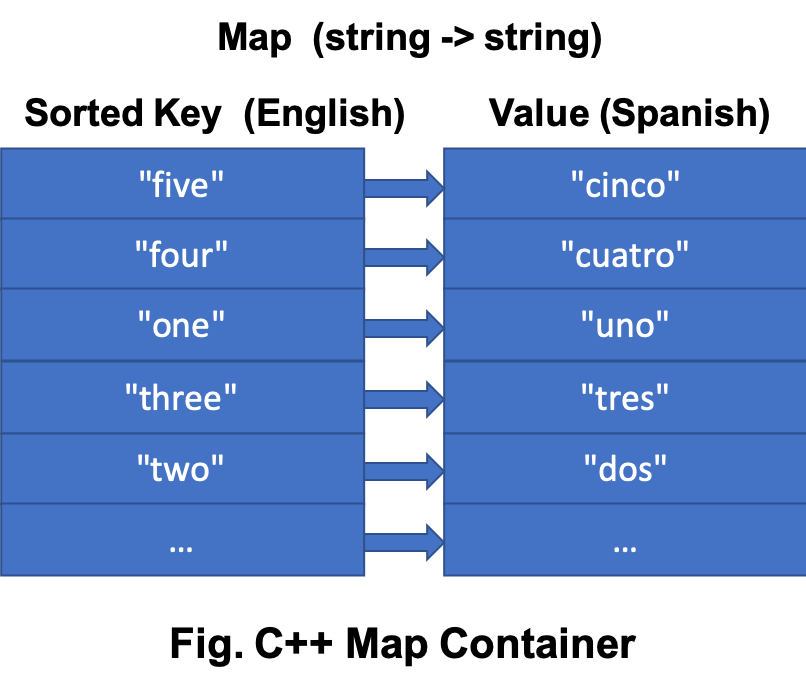
\includegraphics{resources/Map.png}

\begin{itemize}
\tightlist
\item
  keys are mapped to values (one-way)

  \begin{itemize}
  \tightlist
  \item
    values are not mapped to the keys
  \end{itemize}
\item
  under the hood \textbf{map} is implemented as
  \href{https://en.wikipedia.org/wiki/Red\%E2\%80\%93black_tree}{red-black
  trees}
\item
  the complexity (efficiency) of common operations such as search,
  removal, and insertion operations is \(O(log_2 n)\)

  \begin{itemize}
  \tightlist
  \item
    simply put, if there are about 4 billion key-value pairs in a map,
    these common tasks can be completed in about 32 iterations
    (operations)
  \item
    oder of operations is something discussed in more details in Data
    structures and Algorithm courses
  \end{itemize}
\end{itemize}

    \hypertarget{map-objects}{%
\subsection{Map objects}\label{map-objects}}

\begin{itemize}
\tightlist
\item
  must include header file \textbf{\textless map\textgreater{}} and use
  namespace std
\item
  a template class designed to store key of any data type that can be
  compared

  \begin{itemize}
  \tightlist
  \item
    value can be of any type
  \end{itemize}
\item
  map objects must be declared before they can be used
\item
  syntax
\end{itemize}

\begin{Shaded}
\begin{Highlighting}[]
\NormalTok{map}\OperatorTok{\textless{}}\NormalTok{type}\OperatorTok{,}\NormalTok{ type}\OperatorTok{\textgreater{}}\NormalTok{ object}\OperatorTok{;}
\end{Highlighting}
\end{Shaded}

    \begin{tcolorbox}[breakable, size=fbox, boxrule=1pt, pad at break*=1mm,colback=cellbackground, colframe=cellborder]
\prompt{In}{incolor}{1}{\boxspacing}
\begin{Verbatim}[commandchars=\\\{\}]
\PY{c+c1}{// include header files}
\PY{c+cp}{\PYZsh{}}\PY{c+cp}{include} \PY{c+cpf}{\PYZlt{}iostream\PYZgt{}}
\PY{c+cp}{\PYZsh{}}\PY{c+cp}{include} \PY{c+cpf}{\PYZlt{}string\PYZgt{}}
\PY{c+cp}{\PYZsh{}}\PY{c+cp}{include} \PY{c+cpf}{\PYZlt{}map\PYZgt{}}

\PY{k}{using} \PY{k}{namespace} \PY{n+nn}{std}\PY{p}{;}
\end{Verbatim}
\end{tcolorbox}

    \begin{tcolorbox}[breakable, size=fbox, boxrule=1pt, pad at break*=1mm,colback=cellbackground, colframe=cellborder]
\prompt{In}{incolor}{4}{\boxspacing}
\begin{Verbatim}[commandchars=\\\{\}]
\PY{c+c1}{// declare map containers without initialization}
\PY{n}{map}\PY{o}{\PYZlt{}}\PY{n}{string}\PY{p}{,} \PY{n}{string}\PY{o}{\PYZgt{}} \PY{n}{eng2Span}\PY{p}{;}
\PY{n}{map}\PY{o}{\PYZlt{}}\PY{k+kt}{char}\PY{p}{,} \PY{k+kt}{int}\PY{o}{\PYZgt{}} \PY{n}{charToNum}\PY{p}{;}
\PY{n}{map}\PY{o}{\PYZlt{}}\PY{k+kt}{int}\PY{p}{,} \PY{k+kt}{char}\PY{o}{\PYZgt{}} \PY{n}{numToChar}\PY{p}{;}
\end{Verbatim}
\end{tcolorbox}

    \begin{tcolorbox}[breakable, size=fbox, boxrule=1pt, pad at break*=1mm,colback=cellbackground, colframe=cellborder]
\prompt{In}{incolor}{ }{\boxspacing}
\begin{Verbatim}[commandchars=\\\{\}]
\PY{c+c1}{// declare and initialize}
\PY{n}{map}\PY{o}{\PYZlt{}}\PY{n}{string}\PY{p}{,} \PY{k+kt}{int}\PY{o}{\PYZgt{}} \PY{n}{words} \PY{o}{=} \PY{p}{\PYZob{}}
        \PY{p}{\PYZob{}}\PY{l+s}{\PYZdq{}}\PY{l+s}{i}\PY{l+s}{\PYZdq{}}\PY{p}{,} \PY{l+m+mi}{10}\PY{p}{\PYZcb{}}\PY{p}{,}
        \PY{p}{\PYZob{}}\PY{l+s}{\PYZdq{}}\PY{l+s}{love}\PY{l+s}{\PYZdq{}}\PY{p}{,} \PY{l+m+mi}{20}\PY{p}{\PYZcb{}}\PY{p}{,}
        \PY{p}{\PYZob{}}\PY{l+s}{\PYZdq{}}\PY{l+s}{C++}\PY{l+s}{\PYZdq{}}\PY{p}{,} \PY{l+m+mi}{30}\PY{p}{\PYZcb{}}\PY{p}{,}
        \PY{p}{\PYZob{}}\PY{l+s}{\PYZdq{}}\PY{l+s}{!}\PY{l+s}{\PYZdq{}}\PY{p}{,} \PY{l+m+mi}{40}\PY{p}{\PYZcb{}}\PY{p}{,}
    \PY{p}{\PYZcb{}}\PY{p}{;}
\PY{n}{map}\PY{o}{\PYZlt{}}\PY{n}{string}\PY{p}{,} \PY{k+kt}{float}\PY{o}{\PYZgt{}} \PY{n}{prices} \PY{o}{=} \PY{p}{\PYZob{}}\PY{p}{\PYZob{}}\PY{l+s}{\PYZdq{}}\PY{l+s}{apple}\PY{l+s}{\PYZdq{}}\PY{p}{,} \PY{l+m+mf}{1.99}\PY{p}{\PYZcb{}}\PY{p}{,} \PY{p}{\PYZob{}}\PY{l+s}{\PYZdq{}}\PY{l+s}{orange}\PY{l+s}{\PYZdq{}}\PY{p}{,} \PY{l+m+mf}{1.99}\PY{p}{\PYZcb{}}\PY{p}{,} \PY{p}{\PYZob{}}\PY{l+s}{\PYZdq{}}\PY{l+s}{banana}\PY{l+s}{\PYZdq{}}\PY{p}{,} \PY{l+m+mf}{2.99}\PY{p}{\PYZcb{}}\PY{p}{,} \PY{p}{\PYZob{}}\PY{l+s}{\PYZdq{}}\PY{l+s}{lobster}\PY{l+s}{\PYZdq{}}\PY{p}{,} \PY{l+m+mf}{20.85}\PY{p}{\PYZcb{}}\PY{p}{\PYZcb{}}\PY{p}{;}
\PY{n}{map}\PY{o}{\PYZlt{}}\PY{n}{string}\PY{p}{,} \PY{k+kt}{float}\PY{o}{\PYZgt{}} \PY{n}{dupPrices} \PY{o}{=} \PY{n}{prices}\PY{p}{;}
\end{Verbatim}
\end{tcolorbox}

    \begin{tcolorbox}[breakable, size=fbox, boxrule=1pt, pad at break*=1mm,colback=cellbackground, colframe=cellborder]
\prompt{In}{incolor}{16}{\boxspacing}
\begin{Verbatim}[commandchars=\\\{\}]
\PY{c+c1}{// contents of words}
\PY{n}{words}
\end{Verbatim}
\end{tcolorbox}

            \begin{tcolorbox}[breakable, size=fbox, boxrule=.5pt, pad at break*=1mm, opacityfill=0]
\prompt{Out}{outcolor}{16}{\boxspacing}
\begin{Verbatim}[commandchars=\\\{\}]
\{ "!" => 40, "C++" => 30, "i" => 10, "love" => 20 \}
\end{Verbatim}
\end{tcolorbox}
        
    \begin{tcolorbox}[breakable, size=fbox, boxrule=1pt, pad at break*=1mm,colback=cellbackground, colframe=cellborder]
\prompt{In}{incolor}{17}{\boxspacing}
\begin{Verbatim}[commandchars=\\\{\}]
\PY{c+c1}{// prices contents: }
\PY{n}{prices}
\end{Verbatim}
\end{tcolorbox}

            \begin{tcolorbox}[breakable, size=fbox, boxrule=.5pt, pad at break*=1mm, opacityfill=0]
\prompt{Out}{outcolor}{17}{\boxspacing}
\begin{Verbatim}[commandchars=\\\{\}]
\{ "apple" => 1.99000f, "ball" => 0.00000f, "banana" => 2.99000f, "lobster" =>
20.8500f, "orange" => 1.99000f \}
\end{Verbatim}
\end{tcolorbox}
        
    \hypertarget{values-can-be-user-defined-type}{%
\subsubsection{values can be user-defined
type}\label{values-can-be-user-defined-type}}

    \begin{tcolorbox}[breakable, size=fbox, boxrule=1pt, pad at break*=1mm,colback=cellbackground, colframe=cellborder]
\prompt{In}{incolor}{8}{\boxspacing}
\begin{Verbatim}[commandchars=\\\{\}]
\PY{c+c1}{// define Rectangle type}
\PY{c+c1}{// Note \PYZhy{} the word Type is redundant! Rectangle by itself would mean a type}
\PY{k}{struct} \PY{n+nc}{RectangleType} \PY{p}{\PYZob{}}
    \PY{k+kt}{float} \PY{n}{length}\PY{p}{,} \PY{n}{width}\PY{p}{;}
\PY{p}{\PYZcb{}}\PY{p}{;}
\end{Verbatim}
\end{tcolorbox}

    \begin{tcolorbox}[breakable, size=fbox, boxrule=1pt, pad at break*=1mm,colback=cellbackground, colframe=cellborder]
\prompt{In}{incolor}{9}{\boxspacing}
\begin{Verbatim}[commandchars=\\\{\}]
\PY{c+c1}{// create a map that maps ints to RectangleType}
\PY{n}{map}\PY{o}{\PYZlt{}}\PY{k+kt}{int}\PY{p}{,} \PY{n}{RectangleType}\PY{o}{\PYZgt{}} \PY{n}{myRects}\PY{p}{;}
\end{Verbatim}
\end{tcolorbox}

    \begin{tcolorbox}[breakable, size=fbox, boxrule=1pt, pad at break*=1mm,colback=cellbackground, colframe=cellborder]
\prompt{In}{incolor}{10}{\boxspacing}
\begin{Verbatim}[commandchars=\\\{\}]
\PY{c+c1}{// declare and initialize}
\PY{n}{map}\PY{o}{\PYZlt{}}\PY{k+kt}{char}\PY{p}{,} \PY{n}{RectangleType}\PY{o}{\PYZgt{}} \PY{n}{rectMap} \PY{o}{=} \PY{p}{\PYZob{}}\PY{p}{\PYZob{}}\PY{l+s+sc}{\PYZsq{}}\PY{l+s+sc}{A}\PY{l+s+sc}{\PYZsq{}}\PY{p}{,} \PY{p}{\PYZob{}}\PY{l+m+mi}{20}\PY{p}{,} \PY{l+m+mi}{10}\PY{p}{\PYZcb{}}\PY{p}{\PYZcb{}}\PY{p}{,} \PY{p}{\PYZob{}}\PY{l+s+sc}{\PYZsq{}}\PY{l+s+sc}{x}\PY{l+s+sc}{\PYZsq{}}\PY{p}{,} \PY{p}{\PYZob{}}\PY{l+m+mf}{3.5}\PY{p}{,} \PY{l+m+mf}{2.1}\PY{p}{\PYZcb{}}\PY{p}{\PYZcb{}}\PY{p}{\PYZcb{}}\PY{p}{;}
\end{Verbatim}
\end{tcolorbox}

    \hypertarget{accessing-existing-elements}{%
\subsection{Accessing existing
elements}\label{accessing-existing-elements}}

\begin{itemize}
\tightlist
\item
  elements are accessed using keys and NOT the values

  \begin{itemize}
  \tightlist
  \item
    must know the key to get the corresponding values
  \item
    can't get key from its value
  \end{itemize}
\item
  \textbf{at(key)} : access specified element with bounds checking
\item
  \textbf{operator{[}key{]}} : access or insert specified element based
  on key
\item
  similar to vector, but use actual key not index
\end{itemize}

    \begin{tcolorbox}[breakable, size=fbox, boxrule=1pt, pad at break*=1mm,colback=cellbackground, colframe=cellborder]
\prompt{In}{incolor}{11}{\boxspacing}
\begin{Verbatim}[commandchars=\\\{\}]
\PY{c+c1}{// accessing elements using [] bracket operator}
\PY{n}{cout} \PY{o}{\PYZlt{}}\PY{o}{\PYZlt{}} \PY{l+s}{\PYZdq{}}\PY{l+s}{love = }\PY{l+s}{\PYZdq{}} \PY{o}{\PYZlt{}}\PY{o}{\PYZlt{}} \PY{n}{words}\PY{p}{[}\PY{l+s}{\PYZdq{}}\PY{l+s}{love}\PY{l+s}{\PYZdq{}}\PY{p}{]} \PY{o}{\PYZlt{}}\PY{o}{\PYZlt{}} \PY{n}{endl}\PY{p}{;}
\PY{n}{cout} \PY{o}{\PYZlt{}}\PY{o}{\PYZlt{}} \PY{l+s}{\PYZdq{}}\PY{l+s}{apple = }\PY{l+s}{\PYZdq{}} \PY{o}{\PYZlt{}}\PY{o}{\PYZlt{}} \PY{n}{prices}\PY{p}{[}\PY{l+s}{\PYZdq{}}\PY{l+s}{apple}\PY{l+s}{\PYZdq{}}\PY{p}{]} \PY{o}{\PYZlt{}}\PY{o}{\PYZlt{}} \PY{n}{endl}\PY{p}{;}
\PY{n}{cout} \PY{o}{\PYZlt{}}\PY{o}{\PYZlt{}} \PY{l+s}{\PYZdq{}}\PY{l+s}{ball = }\PY{l+s}{\PYZdq{}} \PY{o}{\PYZlt{}}\PY{o}{\PYZlt{}} \PY{n}{prices}\PY{p}{[}\PY{l+s}{\PYZdq{}}\PY{l+s}{ball}\PY{l+s}{\PYZdq{}}\PY{p}{]} \PY{o}{\PYZlt{}}\PY{o}{\PYZlt{}} \PY{n}{endl}\PY{p}{;} \PY{c+c1}{// \PYZdq{}ball doesn\PYZsq{}t exist; returns 0\PYZdq{}}
\end{Verbatim}
\end{tcolorbox}

    \begin{Verbatim}[commandchars=\\\{\}]
love = 20
apple = 1.99
ball = 0
    \end{Verbatim}

            \begin{tcolorbox}[breakable, size=fbox, boxrule=.5pt, pad at break*=1mm, opacityfill=0]
\prompt{Out}{outcolor}{11}{\boxspacing}
\begin{Verbatim}[commandchars=\\\{\}]
@0x105af2ec0
\end{Verbatim}
\end{tcolorbox}
        
    \begin{tcolorbox}[breakable, size=fbox, boxrule=1pt, pad at break*=1mm,colback=cellbackground, colframe=cellborder]
\prompt{In}{incolor}{20}{\boxspacing}
\begin{Verbatim}[commandchars=\\\{\}]
\PY{c+c1}{// key must exist; value is unpredictable if key doesn\PYZsq{}t exist}
\PY{n}{cout} \PY{o}{\PYZlt{}}\PY{o}{\PYZlt{}} \PY{l+s}{\PYZdq{}}\PY{l+s}{cost of kite = }\PY{l+s}{\PYZdq{}} \PY{o}{\PYZlt{}}\PY{o}{\PYZlt{}} \PY{n}{prices}\PY{p}{[}\PY{l+s}{\PYZdq{}}\PY{l+s}{kite}\PY{l+s}{\PYZdq{}}\PY{p}{]}\PY{p}{;}
\end{Verbatim}
\end{tcolorbox}

    \begin{Verbatim}[commandchars=\\\{\}]
cost of kite = 0
    \end{Verbatim}

    \begin{tcolorbox}[breakable, size=fbox, boxrule=1pt, pad at break*=1mm,colback=cellbackground, colframe=cellborder]
\prompt{In}{incolor}{12}{\boxspacing}
\begin{Verbatim}[commandchars=\\\{\}]
\PY{c+c1}{// accessing elements using at() member function}
\PY{n}{cout} \PY{o}{\PYZlt{}}\PY{o}{\PYZlt{}} \PY{l+s}{\PYZdq{}}\PY{l+s}{love = }\PY{l+s}{\PYZdq{}} \PY{o}{\PYZlt{}}\PY{o}{\PYZlt{}} \PY{n}{words}\PY{p}{.}\PY{n}{at}\PY{p}{(}\PY{l+s}{\PYZdq{}}\PY{l+s}{love}\PY{l+s}{\PYZdq{}}\PY{p}{)} \PY{o}{\PYZlt{}}\PY{o}{\PYZlt{}} \PY{n}{endl}\PY{p}{;}
\PY{n}{cout} \PY{o}{\PYZlt{}}\PY{o}{\PYZlt{}} \PY{l+s}{\PYZdq{}}\PY{l+s}{apple = }\PY{l+s}{\PYZdq{}} \PY{o}{\PYZlt{}}\PY{o}{\PYZlt{}} \PY{n}{prices}\PY{p}{.}\PY{n}{at}\PY{p}{(}\PY{l+s}{\PYZdq{}}\PY{l+s}{apple}\PY{l+s}{\PYZdq{}}\PY{p}{)} \PY{o}{\PYZlt{}}\PY{o}{\PYZlt{}} \PY{n}{endl}\PY{p}{;}
\PY{n}{cout} \PY{o}{\PYZlt{}}\PY{o}{\PYZlt{}} \PY{l+s}{\PYZdq{}}\PY{l+s}{ball = }\PY{l+s}{\PYZdq{}} \PY{o}{\PYZlt{}}\PY{o}{\PYZlt{}} \PY{n}{prices}\PY{p}{.}\PY{n}{at}\PY{p}{(}\PY{l+s}{\PYZdq{}}\PY{l+s}{ball}\PY{l+s}{\PYZdq{}}\PY{p}{)} \PY{o}{\PYZlt{}}\PY{o}{\PYZlt{}} \PY{n}{endl}\PY{p}{;} \PY{c+c1}{// \PYZdq{}ball doesn\PYZsq{}t exist; returns 0\PYZdq{}}
\end{Verbatim}
\end{tcolorbox}

    \begin{Verbatim}[commandchars=\\\{\}]
love = 20
apple = 1.99
ball = 0
    \end{Verbatim}

            \begin{tcolorbox}[breakable, size=fbox, boxrule=.5pt, pad at break*=1mm, opacityfill=0]
\prompt{Out}{outcolor}{12}{\boxspacing}
\begin{Verbatim}[commandchars=\\\{\}]
@0x105af2ec0
\end{Verbatim}
\end{tcolorbox}
        
    \begin{tcolorbox}[breakable, size=fbox, boxrule=1pt, pad at break*=1mm,colback=cellbackground, colframe=cellborder]
\prompt{In}{incolor}{21}{\boxspacing}
\begin{Verbatim}[commandchars=\\\{\}]
\PY{c+c1}{// key must exist; value is unpredictable if key doesn\PYZsq{}t exist}
\PY{n}{cout} \PY{o}{\PYZlt{}}\PY{o}{\PYZlt{}} \PY{l+s}{\PYZdq{}}\PY{l+s}{cost of kite = }\PY{l+s}{\PYZdq{}} \PY{o}{\PYZlt{}}\PY{o}{\PYZlt{}} \PY{n}{prices}\PY{p}{.}\PY{n}{at}\PY{p}{(}\PY{l+s}{\PYZdq{}}\PY{l+s}{kite}\PY{l+s}{\PYZdq{}}\PY{p}{)}\PY{p}{;}
\end{Verbatim}
\end{tcolorbox}

    \begin{Verbatim}[commandchars=\\\{\}]
cost of kite = 0
    \end{Verbatim}

    \begin{tcolorbox}[breakable, size=fbox, boxrule=1pt, pad at break*=1mm,colback=cellbackground, colframe=cellborder]
\prompt{In}{incolor}{14}{\boxspacing}
\begin{Verbatim}[commandchars=\\\{\}]
\PY{c+c1}{// declared above, but should be empty map}
\PY{n}{eng2Span}
\end{Verbatim}
\end{tcolorbox}

            \begin{tcolorbox}[breakable, size=fbox, boxrule=.5pt, pad at break*=1mm, opacityfill=0]
\prompt{Out}{outcolor}{14}{\boxspacing}
\begin{Verbatim}[commandchars=\\\{\}]
\{\}
\end{Verbatim}
\end{tcolorbox}
        
    \begin{tcolorbox}[breakable, size=fbox, boxrule=1pt, pad at break*=1mm,colback=cellbackground, colframe=cellborder]
\prompt{In}{incolor}{24}{\boxspacing}
\begin{Verbatim}[commandchars=\\\{\}]
\PY{c+c1}{// accessing user\PYZhy{}defined type as value}
\PY{n}{rectMap}\PY{p}{[}\PY{l+s+sc}{\PYZsq{}}\PY{l+s+sc}{x}\PY{l+s+sc}{\PYZsq{}}\PY{p}{]}\PY{p}{.}\PY{n}{length}
\end{Verbatim}
\end{tcolorbox}

            \begin{tcolorbox}[breakable, size=fbox, boxrule=.5pt, pad at break*=1mm, opacityfill=0]
\prompt{Out}{outcolor}{24}{\boxspacing}
\begin{Verbatim}[commandchars=\\\{\}]
3.50000f
\end{Verbatim}
\end{tcolorbox}
        
    \begin{tcolorbox}[breakable, size=fbox, boxrule=1pt, pad at break*=1mm,colback=cellbackground, colframe=cellborder]
\prompt{In}{incolor}{25}{\boxspacing}
\begin{Verbatim}[commandchars=\\\{\}]
\PY{n}{cout} \PY{o}{\PYZlt{}}\PY{o}{\PYZlt{}} \PY{l+s}{\PYZdq{}}\PY{l+s}{area of rectangle x = }\PY{l+s}{\PYZdq{}} \PY{o}{\PYZlt{}}\PY{o}{\PYZlt{}} \PY{n}{rectMap}\PY{p}{[}\PY{l+s+sc}{\PYZsq{}}\PY{l+s+sc}{x}\PY{l+s+sc}{\PYZsq{}}\PY{p}{]}\PY{p}{.}\PY{n}{length} \PY{o}{*} \PY{n}{rectMap}\PY{p}{[}\PY{l+s+sc}{\PYZsq{}}\PY{l+s+sc}{x}\PY{l+s+sc}{\PYZsq{}}\PY{p}{]}\PY{p}{.}\PY{n}{width}\PY{p}{;}
\end{Verbatim}
\end{tcolorbox}

    \begin{Verbatim}[commandchars=\\\{\}]
area of rectangle x = 7.35
    \end{Verbatim}

    \hypertarget{inserting-key-value-pairs}{%
\subsubsection{inserting key-\textgreater value
pairs}\label{inserting-key-value-pairs}}

\begin{itemize}
\tightlist
\item
  new key value pairs can be inserted to a map container
\item
  if the key exists, existing value will be replaced with the new value
\item
  if the key doesn't exist, new key-value pair will be inserted in the
  right location making sure keys are always sorted
\end{itemize}

    \begin{tcolorbox}[breakable, size=fbox, boxrule=1pt, pad at break*=1mm,colback=cellbackground, colframe=cellborder]
\prompt{In}{incolor}{26}{\boxspacing}
\begin{Verbatim}[commandchars=\\\{\}]
\PY{c+c1}{// add new elements}
\PY{n}{eng2Span}\PY{p}{[}\PY{l+s}{\PYZdq{}}\PY{l+s}{one}\PY{l+s}{\PYZdq{}}\PY{p}{]} \PY{o}{=} \PY{l+s}{\PYZdq{}}\PY{l+s}{uno}\PY{l+s}{\PYZdq{}}\PY{p}{;}
\PY{n}{eng2Span}\PY{p}{[}\PY{l+s}{\PYZdq{}}\PY{l+s}{two}\PY{l+s}{\PYZdq{}}\PY{p}{]} \PY{o}{=} \PY{l+s}{\PYZdq{}}\PY{l+s}{dos}\PY{l+s}{\PYZdq{}}\PY{p}{;}
\PY{n}{eng2Span}\PY{p}{[}\PY{l+s}{\PYZdq{}}\PY{l+s}{three}\PY{l+s}{\PYZdq{}}\PY{p}{]} \PY{o}{=} \PY{l+s}{\PYZdq{}}\PY{l+s}{tres}\PY{l+s}{\PYZdq{}}\PY{p}{;}
\PY{n}{eng2Span}\PY{p}{[}\PY{l+s}{\PYZdq{}}\PY{l+s}{four}\PY{l+s}{\PYZdq{}}\PY{p}{]} \PY{o}{=} \PY{l+s}{\PYZdq{}}\PY{l+s}{cuatro}\PY{l+s}{\PYZdq{}}\PY{p}{;}
\PY{n}{eng2Span}\PY{p}{[}\PY{l+s}{\PYZdq{}}\PY{l+s}{five}\PY{l+s}{\PYZdq{}}\PY{p}{]} \PY{o}{=} \PY{l+s}{\PYZdq{}}\PY{l+s}{sinco}\PY{l+s}{\PYZdq{}}\PY{p}{;}
\end{Verbatim}
\end{tcolorbox}

    \begin{tcolorbox}[breakable, size=fbox, boxrule=1pt, pad at break*=1mm,colback=cellbackground, colframe=cellborder]
\prompt{In}{incolor}{27}{\boxspacing}
\begin{Verbatim}[commandchars=\\\{\}]
\PY{n}{eng2Span} \PY{c+c1}{// sorted based on key}
\end{Verbatim}
\end{tcolorbox}

            \begin{tcolorbox}[breakable, size=fbox, boxrule=.5pt, pad at break*=1mm, opacityfill=0]
\prompt{Out}{outcolor}{27}{\boxspacing}
\begin{Verbatim}[commandchars=\\\{\}]
\{ "five" => "sinco", "four" => "cuatro", "one" => "uno", "three" => "tres",
"two" => "dos" \}
\end{Verbatim}
\end{tcolorbox}
        
    \begin{tcolorbox}[breakable, size=fbox, boxrule=1pt, pad at break*=1mm,colback=cellbackground, colframe=cellborder]
\prompt{In}{incolor}{28}{\boxspacing}
\begin{Verbatim}[commandchars=\\\{\}]
\PY{c+c1}{// sinco is misspelled; let\PYZsq{}s correct its spelling}
\PY{n}{eng2Span}\PY{p}{[}\PY{l+s}{\PYZdq{}}\PY{l+s}{five}\PY{l+s}{\PYZdq{}}\PY{p}{]} \PY{o}{=} \PY{l+s}{\PYZdq{}}\PY{l+s}{cinco}\PY{l+s}{\PYZdq{}}\PY{p}{;}
\end{Verbatim}
\end{tcolorbox}

    \begin{tcolorbox}[breakable, size=fbox, boxrule=1pt, pad at break*=1mm,colback=cellbackground, colframe=cellborder]
\prompt{In}{incolor}{29}{\boxspacing}
\begin{Verbatim}[commandchars=\\\{\}]
\PY{n}{cout} \PY{o}{\PYZlt{}}\PY{o}{\PYZlt{}} \PY{l+s}{\PYZdq{}}\PY{l+s}{ five in English is }\PY{l+s}{\PYZdq{}} \PY{o}{\PYZlt{}}\PY{o}{\PYZlt{}} \PY{n}{eng2Span}\PY{p}{[}\PY{l+s}{\PYZdq{}}\PY{l+s}{five}\PY{l+s}{\PYZdq{}}\PY{p}{]} \PY{o}{\PYZlt{}}\PY{o}{\PYZlt{}} \PY{l+s}{\PYZdq{}}\PY{l+s}{ in Spanish.}\PY{l+s}{\PYZdq{}}\PY{p}{;}
\end{Verbatim}
\end{tcolorbox}

    \begin{Verbatim}[commandchars=\\\{\}]
 five in English is cinco in Spanish.
    \end{Verbatim}

    \hypertarget{capacity}{%
\subsection{Capacity}\label{capacity}}

\begin{itemize}
\tightlist
\item
  similar to vecotr, map provides member functions to find the capacity
  of map containers
\item
  \textbf{empty()} : checks whethere the container is empty
\item
  \textbf{size()} : returns the number of elements

  \begin{itemize}
  \tightlist
  \item
    recall, each element of map is key-\textgreater value pair
  \end{itemize}
\item
  \textbf{max\_size()} : returns the maximum possible number of elements
\end{itemize}

    \begin{tcolorbox}[breakable, size=fbox, boxrule=1pt, pad at break*=1mm,colback=cellbackground, colframe=cellborder]
\prompt{In}{incolor}{31}{\boxspacing}
\begin{Verbatim}[commandchars=\\\{\}]
\PY{n}{cout} \PY{o}{\PYZlt{}}\PY{o}{\PYZlt{}} \PY{n}{boolalpha}\PY{p}{;} \PY{c+c1}{// convert boolean to text true/false}
\PY{n}{cout} \PY{o}{\PYZlt{}}\PY{o}{\PYZlt{}} \PY{l+s}{\PYZdq{}}\PY{l+s}{is eng2Span empty? }\PY{l+s}{\PYZdq{}} \PY{o}{\PYZlt{}}\PY{o}{\PYZlt{}} \PY{n}{eng2Span}\PY{p}{.}\PY{n}{empty}\PY{p}{(}\PY{p}{)} \PY{o}{\PYZlt{}}\PY{o}{\PYZlt{}} \PY{n}{endl}\PY{p}{;}
\PY{n}{cout} \PY{o}{\PYZlt{}}\PY{o}{\PYZlt{}} \PY{l+s}{\PYZdq{}}\PY{l+s}{is prices map empty? }\PY{l+s}{\PYZdq{}} \PY{o}{\PYZlt{}}\PY{o}{\PYZlt{}} \PY{n}{prices}\PY{p}{.}\PY{n}{empty}\PY{p}{(}\PY{p}{)} \PY{o}{\PYZlt{}}\PY{o}{\PYZlt{}} \PY{n}{endl}\PY{p}{;}
\PY{n}{cout} \PY{o}{\PYZlt{}}\PY{o}{\PYZlt{}} \PY{l+s}{\PYZdq{}}\PY{l+s}{total number of key\PYZhy{}\PYZgt{}value pairs in prices: }\PY{l+s}{\PYZdq{}} \PY{o}{\PYZlt{}}\PY{o}{\PYZlt{}} \PY{n}{prices}\PY{p}{.}\PY{n}{size}\PY{p}{(}\PY{p}{)} \PY{o}{\PYZlt{}}\PY{o}{\PYZlt{}} \PY{n}{endl}\PY{p}{;}
\PY{n}{cout} \PY{o}{\PYZlt{}}\PY{o}{\PYZlt{}} \PY{l+s}{\PYZdq{}}\PY{l+s}{max\PYZus{}size of prices: }\PY{l+s}{\PYZdq{}} \PY{o}{\PYZlt{}}\PY{o}{\PYZlt{}} \PY{n}{prices}\PY{p}{.}\PY{n}{max\PYZus{}size}\PY{p}{(}\PY{p}{)} \PY{o}{\PYZlt{}}\PY{o}{\PYZlt{}} \PY{n}{endl}\PY{p}{;}
\end{Verbatim}
\end{tcolorbox}

    \begin{Verbatim}[commandchars=\\\{\}]
is eng2Span empty? false
is prices map empty? false
total number of key->value pairs in prices: 6
max\_size of prices: 288230376151711743
    \end{Verbatim}

    \hypertarget{modifying-maps}{%
\subsection{Modifying maps}\label{modifying-maps}}

\begin{itemize}
\tightlist
\item
  map objects also provide some member functions to modify the contents
  of the containers
\item
  \textbf{clear()} : clears the contents
\item
  \textbf{{[}key{]}} : modifies value at the specified key
\end{itemize}

    \begin{tcolorbox}[breakable, size=fbox, boxrule=1pt, pad at break*=1mm,colback=cellbackground, colframe=cellborder]
\prompt{In}{incolor}{34}{\boxspacing}
\begin{Verbatim}[commandchars=\\\{\}]
\PY{n}{map}\PY{o}{\PYZlt{}}\PY{n}{string}\PY{p}{,} \PY{k+kt}{int}\PY{o}{\PYZgt{}} \PY{n}{adultsage} \PY{o}{=} \PY{p}{\PYZob{}}\PY{p}{\PYZob{}}\PY{l+s}{\PYZdq{}}\PY{l+s}{John}\PY{l+s}{\PYZdq{}}\PY{p}{,}\PY{l+m+mi}{21}\PY{p}{\PYZcb{}}\PY{p}{,} \PY{p}{\PYZob{}}\PY{l+s}{\PYZdq{}}\PY{l+s}{Maya}\PY{l+s}{\PYZdq{}}\PY{p}{,}\PY{l+m+mi}{74}\PY{p}{\PYZcb{}}\PY{p}{,} \PY{p}{\PYZob{}}\PY{l+s}{\PYZdq{}}\PY{l+s}{Jenny}\PY{l+s}{\PYZdq{}}\PY{p}{,} \PY{l+m+mi}{46}\PY{p}{\PYZcb{}}\PY{p}{,} \PY{p}{\PYZob{}}\PY{l+s}{\PYZdq{}}\PY{l+s}{Jordan}\PY{l+s}{\PYZdq{}}\PY{p}{,} \PY{l+m+mi}{48}\PY{p}{\PYZcb{}}\PY{p}{,} \PY{p}{\PYZob{}}\PY{l+s}{\PYZdq{}}\PY{l+s}{Mike}\PY{l+s}{\PYZdq{}}\PY{p}{,} \PY{l+m+mi}{46}\PY{p}{\PYZcb{}}\PY{p}{\PYZcb{}}\PY{p}{;}
\end{Verbatim}
\end{tcolorbox}

    \begin{tcolorbox}[breakable, size=fbox, boxrule=1pt, pad at break*=1mm,colback=cellbackground, colframe=cellborder]
\prompt{In}{incolor}{36}{\boxspacing}
\begin{Verbatim}[commandchars=\\\{\}]
\PY{n}{cout} \PY{o}{\PYZlt{}}\PY{o}{\PYZlt{}} \PY{n}{adultsage} \PY{o}{\PYZlt{}}\PY{o}{\PYZlt{}} \PY{n}{endl}\PY{p}{;}
\PY{n}{adultsage}\PY{p}{.}\PY{n}{clear}\PY{p}{(}\PY{p}{)}\PY{p}{;} \PY{c+c1}{// delete all the elements}
\end{Verbatim}
\end{tcolorbox}

    \begin{Verbatim}[commandchars=\\\{\}]
\{Jenny:46, John:21, Jordan:48, Maya:74, Mike:46\}
    \end{Verbatim}

    \begin{tcolorbox}[breakable, size=fbox, boxrule=1pt, pad at break*=1mm,colback=cellbackground, colframe=cellborder]
\prompt{In}{incolor}{37}{\boxspacing}
\begin{Verbatim}[commandchars=\\\{\}]
\PY{c+c1}{// should be empty}
\PY{n}{adultsage}
\end{Verbatim}
\end{tcolorbox}

            \begin{tcolorbox}[breakable, size=fbox, boxrule=.5pt, pad at break*=1mm, opacityfill=0]
\prompt{Out}{outcolor}{37}{\boxspacing}
\begin{Verbatim}[commandchars=\\\{\}]
\{\}
\end{Verbatim}
\end{tcolorbox}
        
    \hypertarget{aggregate-comparisons}{%
\subsection{Aggregate comparisons}\label{aggregate-comparisons}}

\begin{itemize}
\tightlist
\item
  comparison operators ==, !=, \textless, \textgreater, \textless=, and
  \textgreater= are overloaded and works between two maps
\item
  elements are compared lexicographically
\end{itemize}

    \hypertarget{traversing-maps}{%
\subsection{Traversing maps}\label{traversing-maps}}

\begin{itemize}
\tightlist
\item
  map containers can be traveresed from the first element to the last
  (similar to array, string and vector)
\item
  map provides iterators similar to iterators in string or vector

  \begin{itemize}
  \tightlist
  \item
    let's you iterate over all the elements
  \end{itemize}
\item
  iterator of map is a special pointer that has two elements
  \textbf{first} and \textbf{second}

  \begin{itemize}
  \tightlist
  \item
    first is the key and second is the value
  \end{itemize}
\item
  \textbf{begin} - returns an iterator to the beginning (first element)
\item
  \textbf{end} - returns an iterator to the end (past the last element)
\item
  \textbf{rbegin} - returns a reverse iterator to the beginning (past
  the last element)
\item
  \textbf{rend} - returns a reverse iterator to the end (past the first
  element)
\end{itemize}

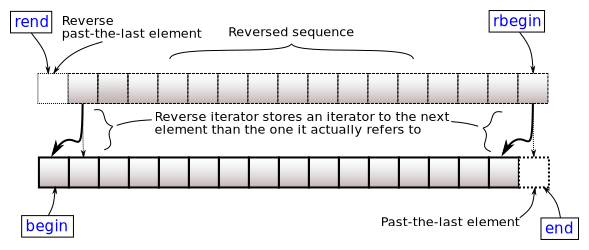
\includegraphics{resources/range-rbegin-rend.png}

    \begin{tcolorbox}[breakable, size=fbox, boxrule=1pt, pad at break*=1mm,colback=cellbackground, colframe=cellborder]
\prompt{In}{incolor}{39}{\boxspacing}
\begin{Verbatim}[commandchars=\\\{\}]
\PY{n}{map}\PY{o}{\PYZlt{}}\PY{k+kt}{int}\PY{p}{,} \PY{n}{string}\PY{o}{\PYZgt{}} \PY{n}{amap} \PY{o}{=} \PY{p}{\PYZob{}}\PY{p}{\PYZob{}}\PY{l+m+mi}{10}\PY{p}{,} \PY{l+s}{\PYZdq{}}\PY{l+s}{val1}\PY{l+s}{\PYZdq{}}\PY{p}{\PYZcb{}}\PY{p}{,} \PY{p}{\PYZob{}}\PY{l+m+mi}{15}\PY{p}{,} \PY{l+s}{\PYZdq{}}\PY{l+s}{val2}\PY{l+s}{\PYZdq{}}\PY{p}{\PYZcb{}}\PY{p}{,} \PY{p}{\PYZob{}}\PY{l+m+mi}{20}\PY{p}{,} \PY{l+s}{\PYZdq{}}\PY{l+s}{val3}\PY{l+s}{\PYZdq{}}\PY{p}{\PYZcb{}}\PY{p}{,} \PY{p}{\PYZob{}}\PY{l+m+mi}{30}\PY{p}{,} \PY{l+s}{\PYZdq{}}\PY{l+s}{val4}\PY{l+s}{\PYZdq{}}\PY{p}{\PYZcb{}}\PY{p}{,} \PY{p}{\PYZob{}}\PY{l+m+mi}{35}\PY{p}{,} \PY{l+s}{\PYZdq{}}\PY{l+s}{val5}\PY{l+s}{\PYZdq{}}\PY{p}{\PYZcb{}}\PY{p}{\PYZcb{}}\PY{p}{;}
\end{Verbatim}
\end{tcolorbox}

    \begin{tcolorbox}[breakable, size=fbox, boxrule=1pt, pad at break*=1mm,colback=cellbackground, colframe=cellborder]
\prompt{In}{incolor}{40}{\boxspacing}
\begin{Verbatim}[commandchars=\\\{\}]
\PY{k}{for}\PY{p}{(}\PY{k}{auto} \PY{n}{iterator} \PY{o}{=} \PY{n}{amap}\PY{p}{.}\PY{n}{begin}\PY{p}{(}\PY{p}{)}\PY{p}{;} \PY{n}{iterator} \PY{o}{!}\PY{o}{=} \PY{n}{amap}\PY{p}{.}\PY{n}{end}\PY{p}{(}\PY{p}{)}\PY{p}{;} \PY{n}{iterator}\PY{o}{+}\PY{o}{+}\PY{p}{)}
    \PY{n}{cout} \PY{o}{\PYZlt{}}\PY{o}{\PYZlt{}} \PY{p}{(}\PY{o}{*}\PY{n}{iterator}\PY{p}{)}\PY{p}{.}\PY{n}{first} \PY{o}{\PYZlt{}}\PY{o}{\PYZlt{}} \PY{l+s}{\PYZdq{}}\PY{l+s}{ =\PYZgt{} }\PY{l+s}{\PYZdq{}} \PY{o}{\PYZlt{}}\PY{o}{\PYZlt{}} \PY{n}{iterator}\PY{o}{\PYZhy{}}\PY{o}{\PYZgt{}}\PY{n}{second} \PY{o}{\PYZlt{}}\PY{o}{\PYZlt{}} \PY{n}{endl}\PY{p}{;}
\end{Verbatim}
\end{tcolorbox}

    \begin{Verbatim}[commandchars=\\\{\}]
10 => val1
15 => val2
20 => val3
30 => val4
35 => val5
    \end{Verbatim}

    \begin{tcolorbox}[breakable, size=fbox, boxrule=1pt, pad at break*=1mm,colback=cellbackground, colframe=cellborder]
\prompt{In}{incolor}{41}{\boxspacing}
\begin{Verbatim}[commandchars=\\\{\}]
\PY{c+c1}{// iterate using range\PYZhy{}based loop}
\PY{k}{for} \PY{p}{(}\PY{k}{auto} \PY{n+nl}{e} \PY{p}{:} \PY{n}{amap}\PY{p}{)}
    \PY{n}{cout} \PY{o}{\PYZlt{}}\PY{o}{\PYZlt{}} \PY{n}{e}\PY{p}{.}\PY{n}{first} \PY{o}{\PYZlt{}}\PY{o}{\PYZlt{}} \PY{l+s}{\PYZdq{}}\PY{l+s}{ \PYZhy{}\PYZgt{} }\PY{l+s}{\PYZdq{}} \PY{o}{\PYZlt{}}\PY{o}{\PYZlt{}} \PY{n}{e}\PY{p}{.}\PY{n}{second} \PY{o}{\PYZlt{}}\PY{o}{\PYZlt{}} \PY{n}{endl}\PY{p}{;}
\end{Verbatim}
\end{tcolorbox}

    \begin{Verbatim}[commandchars=\\\{\}]
10 -> val1
15 -> val2
20 -> val3
30 -> val4
35 -> val5
    \end{Verbatim}

    \begin{tcolorbox}[breakable, size=fbox, boxrule=1pt, pad at break*=1mm,colback=cellbackground, colframe=cellborder]
\prompt{In}{incolor}{27}{\boxspacing}
\begin{Verbatim}[commandchars=\\\{\}]
\PY{c+c1}{// type alias}
\PY{k}{using} \PY{n}{mii} \PY{o}{=} \PY{n}{map}\PY{o}{\PYZlt{}}\PY{k+kt}{int}\PY{p}{,} \PY{k+kt}{int}\PY{o}{\PYZgt{}}\PY{p}{;}
\end{Verbatim}
\end{tcolorbox}

    \begin{tcolorbox}[breakable, size=fbox, boxrule=1pt, pad at break*=1mm,colback=cellbackground, colframe=cellborder]
\prompt{In}{incolor}{28}{\boxspacing}
\begin{Verbatim}[commandchars=\\\{\}]
\PY{n}{mii} \PY{n}{map1} \PY{o}{=} \PY{p}{\PYZob{}}\PY{p}{\PYZob{}}\PY{l+m+mi}{1}\PY{p}{,}\PY{l+m+mi}{10}\PY{p}{\PYZcb{}}\PY{p}{,} \PY{p}{\PYZob{}}\PY{l+m+mi}{2}\PY{p}{,}\PY{l+m+mi}{20}\PY{p}{\PYZcb{}}\PY{p}{,} \PY{p}{\PYZob{}}\PY{l+m+mi}{3}\PY{p}{,}\PY{l+m+mi}{30}\PY{p}{\PYZcb{}}\PY{p}{,} \PY{p}{\PYZob{}}\PY{l+m+mi}{4}\PY{p}{,}\PY{l+m+mi}{40}\PY{p}{\PYZcb{}}\PY{p}{,} \PY{p}{\PYZob{}}\PY{l+m+mi}{5}\PY{p}{,}\PY{l+m+mi}{50}\PY{p}{\PYZcb{}}\PY{p}{\PYZcb{}}\PY{p}{;}
\PY{n}{cout} \PY{o}{\PYZlt{}}\PY{o}{\PYZlt{}} \PY{n}{map1} \PY{o}{\PYZlt{}}\PY{o}{\PYZlt{}} \PY{n}{endl}\PY{p}{;}
\end{Verbatim}
\end{tcolorbox}

    \begin{Verbatim}[commandchars=\\\{\}]
\{1:10, 2:20, 3:30, 4:40, 5:50\}
    \end{Verbatim}

    \hypertarget{lookup-lements}{%
\subsection{Lookup lements}\label{lookup-lements}}

\begin{itemize}
\tightlist
\item
  map containers provide member functions to search for element with
  given key in a map container

  \begin{itemize}
  \tightlist
  \item
    is typically used if you're not sure if a given key exists or not
  \end{itemize}
\item
  \textbf{count(key)} : returns the number of elements matching specific
  key (always 1 if exists, 0 otherwise)
\item
  \textbf{find(key)} : finds elements with specific key, returns
  iterator
\end{itemize}

    \begin{tcolorbox}[breakable, size=fbox, boxrule=1pt, pad at break*=1mm,colback=cellbackground, colframe=cellborder]
\prompt{In}{incolor}{2}{\boxspacing}
\begin{Verbatim}[commandchars=\\\{\}]
\PY{c+c1}{// map char to its ASCII value}
\PY{n}{map}\PY{o}{\PYZlt{}}\PY{k+kt}{char}\PY{p}{,} \PY{k+kt}{int}\PY{o}{\PYZgt{}} \PY{n}{mapci} \PY{o}{=} \PY{p}{\PYZob{}}\PY{p}{\PYZob{}}\PY{l+s+sc}{\PYZsq{}}\PY{l+s+sc}{a}\PY{l+s+sc}{\PYZsq{}}\PY{p}{,} \PY{l+s+sc}{\PYZsq{}}\PY{l+s+sc}{a}\PY{l+s+sc}{\PYZsq{}}\PY{p}{\PYZcb{}}\PY{p}{,} \PY{p}{\PYZob{}}\PY{l+s+sc}{\PYZsq{}}\PY{l+s+sc}{b}\PY{l+s+sc}{\PYZsq{}}\PY{p}{,} \PY{l+s+sc}{\PYZsq{}}\PY{l+s+sc}{b}\PY{l+s+sc}{\PYZsq{}}\PY{p}{\PYZcb{}}\PY{p}{,} \PY{p}{\PYZob{}}\PY{l+s+sc}{\PYZsq{}}\PY{l+s+sc}{c}\PY{l+s+sc}{\PYZsq{}}\PY{p}{,} \PY{l+s+sc}{\PYZsq{}}\PY{l+s+sc}{c}\PY{l+s+sc}{\PYZsq{}}\PY{p}{\PYZcb{}}\PY{p}{,} \PY{p}{\PYZob{}}\PY{l+s+sc}{\PYZsq{}}\PY{l+s+sc}{A}\PY{l+s+sc}{\PYZsq{}}\PY{p}{,} \PY{l+s+sc}{\PYZsq{}}\PY{l+s+sc}{A}\PY{l+s+sc}{\PYZsq{}}\PY{p}{\PYZcb{}}\PY{p}{,} \PY{p}{\PYZob{}}\PY{l+s+sc}{\PYZsq{}}\PY{l+s+sc}{B}\PY{l+s+sc}{\PYZsq{}}\PY{p}{,} \PY{l+s+sc}{\PYZsq{}}\PY{l+s+sc}{B}\PY{l+s+sc}{\PYZsq{}}\PY{p}{\PYZcb{}}\PY{p}{,} \PY{p}{\PYZob{}}\PY{l+s+sc}{\PYZsq{}}\PY{l+s+sc}{1}\PY{l+s+sc}{\PYZsq{}}\PY{p}{,} \PY{l+s+sc}{\PYZsq{}}\PY{l+s+sc}{1}\PY{l+s+sc}{\PYZsq{}}\PY{p}{\PYZcb{}}\PY{p}{\PYZcb{}}\PY{p}{;}
\end{Verbatim}
\end{tcolorbox}

    \begin{tcolorbox}[breakable, size=fbox, boxrule=1pt, pad at break*=1mm,colback=cellbackground, colframe=cellborder]
\prompt{In}{incolor}{3}{\boxspacing}
\begin{Verbatim}[commandchars=\\\{\}]
\PY{n}{mapci}
\end{Verbatim}
\end{tcolorbox}

            \begin{tcolorbox}[breakable, size=fbox, boxrule=.5pt, pad at break*=1mm, opacityfill=0]
\prompt{Out}{outcolor}{3}{\boxspacing}
\begin{Verbatim}[commandchars=\\\{\}]
\{ '1' => 49, 'A' => 65, 'B' => 66, 'a' => 97, 'b' => 98, 'c' => 99 \}
\end{Verbatim}
\end{tcolorbox}
        
    \begin{tcolorbox}[breakable, size=fbox, boxrule=1pt, pad at break*=1mm,colback=cellbackground, colframe=cellborder]
\prompt{In}{incolor}{4}{\boxspacing}
\begin{Verbatim}[commandchars=\\\{\}]
\PY{n}{cout} \PY{o}{\PYZlt{}}\PY{o}{\PYZlt{}} \PY{n}{mapci}\PY{p}{.}\PY{n}{count}\PY{p}{(}\PY{l+s+sc}{\PYZsq{}}\PY{l+s+sc}{a}\PY{l+s+sc}{\PYZsq{}}\PY{p}{)} \PY{o}{\PYZlt{}}\PY{o}{\PYZlt{}} \PY{n}{endl}\PY{p}{;}
\end{Verbatim}
\end{tcolorbox}

    \begin{Verbatim}[commandchars=\\\{\}]
1
    \end{Verbatim}

    \begin{tcolorbox}[breakable, size=fbox, boxrule=1pt, pad at break*=1mm,colback=cellbackground, colframe=cellborder]
\prompt{In}{incolor}{5}{\boxspacing}
\begin{Verbatim}[commandchars=\\\{\}]
\PY{n}{cout} \PY{o}{\PYZlt{}}\PY{o}{\PYZlt{}} \PY{n}{mapci}\PY{p}{.}\PY{n}{count}\PY{p}{(}\PY{l+s+sc}{\PYZsq{}}\PY{l+s+sc}{z}\PY{l+s+sc}{\PYZsq{}}\PY{p}{)} \PY{o}{\PYZlt{}}\PY{o}{\PYZlt{}} \PY{n}{endl}\PY{p}{;}
\end{Verbatim}
\end{tcolorbox}

    \begin{Verbatim}[commandchars=\\\{\}]
0
    \end{Verbatim}

    \begin{tcolorbox}[breakable, size=fbox, boxrule=1pt, pad at break*=1mm,colback=cellbackground, colframe=cellborder]
\prompt{In}{incolor}{6}{\boxspacing}
\begin{Verbatim}[commandchars=\\\{\}]
\PY{k}{if} \PY{p}{(}\PY{n}{mapci}\PY{p}{.}\PY{n}{count}\PY{p}{(}\PY{l+s+sc}{\PYZsq{}}\PY{l+s+sc}{a}\PY{l+s+sc}{\PYZsq{}}\PY{p}{)} \PY{o}{=}\PY{o}{=} \PY{l+m+mi}{1}\PY{p}{)}
    \PY{n}{cout} \PY{o}{\PYZlt{}}\PY{o}{\PYZlt{}} \PY{l+s}{\PYZdq{}}\PY{l+s}{Found!}\PY{l+s}{\PYZdq{}}\PY{p}{;}
\PY{k}{else}
    \PY{n}{cout} \PY{o}{\PYZlt{}}\PY{o}{\PYZlt{}} \PY{l+s}{\PYZdq{}}\PY{l+s}{Not found!}\PY{l+s}{\PYZdq{}}\PY{p}{;}
\end{Verbatim}
\end{tcolorbox}

    \begin{Verbatim}[commandchars=\\\{\}]
Found!
    \end{Verbatim}

    \begin{tcolorbox}[breakable, size=fbox, boxrule=1pt, pad at break*=1mm,colback=cellbackground, colframe=cellborder]
\prompt{In}{incolor}{7}{\boxspacing}
\begin{Verbatim}[commandchars=\\\{\}]
\PY{c+c1}{// find method; returns iterator}
\PY{k}{auto} \PY{n}{it} \PY{o}{=} \PY{n}{mapci}\PY{p}{.}\PY{n}{find}\PY{p}{(}\PY{l+s+sc}{\PYZsq{}}\PY{l+s+sc}{c}\PY{l+s+sc}{\PYZsq{}}\PY{p}{)}\PY{p}{;}
\PY{k}{if} \PY{p}{(}\PY{n}{it} \PY{o}{!}\PY{o}{=} \PY{n}{mapci}\PY{p}{.}\PY{n}{end}\PY{p}{(}\PY{p}{)}\PY{p}{)}
    \PY{n}{cout} \PY{o}{\PYZlt{}}\PY{o}{\PYZlt{}} \PY{l+s}{\PYZdq{}}\PY{l+s}{found }\PY{l+s}{\PYZdq{}} \PY{o}{\PYZlt{}}\PY{o}{\PYZlt{}} \PY{n}{it}\PY{o}{\PYZhy{}}\PY{o}{\PYZgt{}}\PY{n}{first} \PY{o}{\PYZlt{}}\PY{o}{\PYZlt{}} \PY{l+s}{\PYZdq{}}\PY{l+s}{ =\PYZgt{} }\PY{l+s}{\PYZdq{}} \PY{o}{\PYZlt{}}\PY{o}{\PYZlt{}} \PY{n}{it}\PY{o}{\PYZhy{}}\PY{o}{\PYZgt{}}\PY{n}{second} \PY{o}{\PYZlt{}}\PY{o}{\PYZlt{}} \PY{n}{endl}\PY{p}{;}
\PY{k}{else}
    \PY{n}{cout} \PY{o}{\PYZlt{}}\PY{o}{\PYZlt{}} \PY{l+s}{\PYZdq{}}\PY{l+s}{NOT found!}\PY{l+s}{\PYZdq{}}\PY{p}{;}
\end{Verbatim}
\end{tcolorbox}

    \begin{Verbatim}[commandchars=\\\{\}]
found c => 99
    \end{Verbatim}

    \begin{tcolorbox}[breakable, size=fbox, boxrule=1pt, pad at break*=1mm,colback=cellbackground, colframe=cellborder]
\prompt{In}{incolor}{8}{\boxspacing}
\begin{Verbatim}[commandchars=\\\{\}]
\PY{c+c1}{// erase using iterator}
\PY{n}{it} \PY{o}{=} \PY{n}{mapci}\PY{p}{.}\PY{n}{erase}\PY{p}{(}\PY{n}{it}\PY{p}{)}\PY{p}{;}
\end{Verbatim}
\end{tcolorbox}

    \begin{tcolorbox}[breakable, size=fbox, boxrule=1pt, pad at break*=1mm,colback=cellbackground, colframe=cellborder]
\prompt{In}{incolor}{9}{\boxspacing}
\begin{Verbatim}[commandchars=\\\{\}]
\PY{c+c1}{// it points to key \PYZsq{}c\PYZsq{}, so it must be erased}
\PY{n}{mapci}
\end{Verbatim}
\end{tcolorbox}

            \begin{tcolorbox}[breakable, size=fbox, boxrule=.5pt, pad at break*=1mm, opacityfill=0]
\prompt{Out}{outcolor}{9}{\boxspacing}
\begin{Verbatim}[commandchars=\\\{\}]
\{ '1' => 49, 'A' => 65, 'B' => 66, 'a' => 97, 'b' => 98 \}
\end{Verbatim}
\end{tcolorbox}
        
    \hypertarget{passing-map-objects-to-functions}{%
\subsection{Passing map objects to
functions}\label{passing-map-objects-to-functions}}

\begin{itemize}
\tightlist
\item
  map objects can be passed by value and by reference

  \begin{itemize}
  \tightlist
  \item
    by reference is preferred to prevent copying all the elements unless
    it's necessary
  \end{itemize}
\end{itemize}

    \begin{tcolorbox}[breakable, size=fbox, boxrule=1pt, pad at break*=1mm,colback=cellbackground, colframe=cellborder]
\prompt{In}{incolor}{18}{\boxspacing}
\begin{Verbatim}[commandchars=\\\{\}]
\PY{c+c1}{// linear search function that returns true if key is found in someMap}
\PY{k+kt}{bool} \PY{n+nf}{searchMap}\PY{p}{(}\PY{k}{const} \PY{n}{map}\PY{o}{\PYZlt{}}\PY{k+kt}{char}\PY{p}{,} \PY{k+kt}{int}\PY{o}{\PYZgt{}} \PY{o}{\PYZam{}} \PY{n}{someMap}\PY{p}{,} \PY{k+kt}{char} \PY{n}{key}\PY{p}{)} \PY{p}{\PYZob{}}
    \PY{k}{auto} \PY{n}{it} \PY{o}{=} \PY{n}{someMap}\PY{p}{.}\PY{n}{find}\PY{p}{(}\PY{n}{key}\PY{p}{)}\PY{p}{;}
    \PY{k}{return} \PY{n}{it} \PY{o}{!}\PY{o}{=} \PY{n}{someMap}\PY{p}{.}\PY{n}{end}\PY{p}{(}\PY{p}{)}\PY{p}{;}
\PY{p}{\PYZcb{}}
\end{Verbatim}
\end{tcolorbox}

    \begin{tcolorbox}[breakable, size=fbox, boxrule=1pt, pad at break*=1mm,colback=cellbackground, colframe=cellborder]
\prompt{In}{incolor}{20}{\boxspacing}
\begin{Verbatim}[commandchars=\\\{\}]
\PY{n}{cout} \PY{o}{\PYZlt{}}\PY{o}{\PYZlt{}} \PY{n}{boolalpha} \PY{o}{\PYZlt{}}\PY{o}{\PYZlt{}} \PY{l+s}{\PYZdq{}}\PY{l+s}{A exists as key? }\PY{l+s}{\PYZdq{}} \PY{o}{\PYZlt{}}\PY{o}{\PYZlt{}} \PY{n}{searchMap}\PY{p}{(}\PY{n}{mapci}\PY{p}{,} \PY{l+s+sc}{\PYZsq{}}\PY{l+s+sc}{A}\PY{l+s+sc}{\PYZsq{}}\PY{p}{)}\PY{p}{;}
\end{Verbatim}
\end{tcolorbox}

    \begin{Verbatim}[commandchars=\\\{\}]
A exists as key? true
    \end{Verbatim}

    \begin{tcolorbox}[breakable, size=fbox, boxrule=1pt, pad at break*=1mm,colback=cellbackground, colframe=cellborder]
\prompt{In}{incolor}{21}{\boxspacing}
\begin{Verbatim}[commandchars=\\\{\}]
\PY{n}{cout} \PY{o}{\PYZlt{}}\PY{o}{\PYZlt{}} \PY{n}{boolalpha} \PY{o}{\PYZlt{}}\PY{o}{\PYZlt{}} \PY{l+s}{\PYZdq{}}\PY{l+s}{\PYZdl{} exists as key? }\PY{l+s}{\PYZdq{}} \PY{o}{\PYZlt{}}\PY{o}{\PYZlt{}} \PY{n}{searchMap}\PY{p}{(}\PY{n}{mapci}\PY{p}{,} \PY{l+s+sc}{\PYZsq{}}\PY{l+s+sc}{\PYZdl{}}\PY{l+s+sc}{\PYZsq{}}\PY{p}{)}\PY{p}{;}
\end{Verbatim}
\end{tcolorbox}

    \begin{Verbatim}[commandchars=\\\{\}]
\$ exists as key? false
    \end{Verbatim}

    \hypertarget{returning-map-objects-from-functions}{%
\subsection{Returning map objects from
functions}\label{returning-map-objects-from-functions}}

\begin{itemize}
\tightlist
\item
  map objects can be returned from functions
\item
  however, pass by reference is preferred to get the data out of
  function instead of explictly returning a map
\end{itemize}

    \begin{tcolorbox}[breakable, size=fbox, boxrule=1pt, pad at break*=1mm,colback=cellbackground, colframe=cellborder]
\prompt{In}{incolor}{22}{\boxspacing}
\begin{Verbatim}[commandchars=\\\{\}]
\PY{c+c1}{// function updates the map using pass\PYZhy{}by\PYZhy{}reference}
\PY{k+kt}{void} \PY{n+nf}{createMap}\PY{p}{(}\PY{n}{map}\PY{o}{\PYZlt{}}\PY{k+kt}{int}\PY{p}{,} \PY{n}{string}\PY{o}{\PYZgt{}} \PY{o}{\PYZam{}} \PY{n}{m}\PY{p}{)} \PY{p}{\PYZob{}}
    \PY{n}{m}\PY{p}{[}\PY{l+m+mi}{1}\PY{p}{]} \PY{o}{=} \PY{l+s}{\PYZdq{}}\PY{l+s}{one}\PY{l+s}{\PYZdq{}}\PY{p}{;}
    \PY{n}{m}\PY{p}{[}\PY{l+m+mi}{2}\PY{p}{]} \PY{o}{=} \PY{l+s}{\PYZdq{}}\PY{l+s}{two}\PY{l+s}{\PYZdq{}}\PY{p}{;}
    \PY{n}{m}\PY{p}{[}\PY{l+m+mi}{3}\PY{p}{]} \PY{o}{=} \PY{l+s}{\PYZdq{}}\PY{l+s}{three}\PY{l+s}{\PYZdq{}}\PY{p}{;}
    \PY{n}{m}\PY{p}{[}\PY{l+m+mi}{4}\PY{p}{]} \PY{o}{=} \PY{l+s}{\PYZdq{}}\PY{l+s}{four}\PY{l+s}{\PYZdq{}}\PY{p}{;}
    \PY{c+c1}{// ...etc.}
\PY{p}{\PYZcb{}}
\end{Verbatim}
\end{tcolorbox}

    \begin{tcolorbox}[breakable, size=fbox, boxrule=1pt, pad at break*=1mm,colback=cellbackground, colframe=cellborder]
\prompt{In}{incolor}{23}{\boxspacing}
\begin{Verbatim}[commandchars=\\\{\}]
\PY{c+c1}{// create an empty map}
\PY{n}{map}\PY{o}{\PYZlt{}}\PY{k+kt}{int}\PY{p}{,} \PY{n}{string}\PY{o}{\PYZgt{}} \PY{n}{numbers}\PY{p}{;}
\end{Verbatim}
\end{tcolorbox}

    \begin{tcolorbox}[breakable, size=fbox, boxrule=1pt, pad at break*=1mm,colback=cellbackground, colframe=cellborder]
\prompt{In}{incolor}{24}{\boxspacing}
\begin{Verbatim}[commandchars=\\\{\}]
\PY{c+c1}{// let\PYZsq{}s create the map using function}
\PY{n}{createMap}\PY{p}{(}\PY{n}{numbers}\PY{p}{)}\PY{p}{;}
\end{Verbatim}
\end{tcolorbox}

    \begin{tcolorbox}[breakable, size=fbox, boxrule=1pt, pad at break*=1mm,colback=cellbackground, colframe=cellborder]
\prompt{In}{incolor}{26}{\boxspacing}
\begin{Verbatim}[commandchars=\\\{\}]
\PY{c+c1}{// check the contents if the function inserted elements into map}
\PY{n}{numbers}
\end{Verbatim}
\end{tcolorbox}

            \begin{tcolorbox}[breakable, size=fbox, boxrule=.5pt, pad at break*=1mm, opacityfill=0]
\prompt{Out}{outcolor}{26}{\boxspacing}
\begin{Verbatim}[commandchars=\\\{\}]
\{ 1 => "one", 2 => "two", 3 => "three", 4 => "four" \}
\end{Verbatim}
\end{tcolorbox}
        
    

    \hypertarget{applications}{%
\subsection{Applications}\label{applications}}

\begin{itemize}
\tightlist
\item
  map can be applied to many problems \#\#\#\# keep track of menu items
  and the customers who ordered those items
\item
  https://open.kattis.com/problems/baconeggsandspam
\end{itemize}

    \begin{tcolorbox}[breakable, size=fbox, boxrule=1pt, pad at break*=1mm,colback=cellbackground, colframe=cellborder]
\prompt{In}{incolor}{10}{\boxspacing}
\begin{Verbatim}[commandchars=\\\{\}]
\PY{c+cp}{\PYZsh{}}\PY{c+cp}{include} \PY{c+cpf}{\PYZlt{}map\PYZgt{}}
\PY{c+cp}{\PYZsh{}}\PY{c+cp}{include} \PY{c+cpf}{\PYZlt{}vector\PYZgt{}}
\PY{c+cp}{\PYZsh{}}\PY{c+cp}{include} \PY{c+cpf}{\PYZlt{}algorithm\PYZgt{}}
\PY{c+cp}{\PYZsh{}}\PY{c+cp}{include} \PY{c+cpf}{\PYZlt{}string\PYZgt{}}

\PY{k}{using} \PY{k}{namespace} \PY{n+nn}{std}\PY{p}{;}
\end{Verbatim}
\end{tcolorbox}

    \begin{tcolorbox}[breakable, size=fbox, boxrule=1pt, pad at break*=1mm,colback=cellbackground, colframe=cellborder]
\prompt{In}{incolor}{11}{\boxspacing}
\begin{Verbatim}[commandchars=\\\{\}]
\PY{n}{map}\PY{o}{\PYZlt{}}\PY{n}{string}\PY{p}{,} \PY{n}{vector}\PY{o}{\PYZlt{}}\PY{n}{string}\PY{o}{\PYZgt{}} \PY{o}{\PYZgt{}} \PY{n}{items}\PY{p}{;}
\end{Verbatim}
\end{tcolorbox}

    \begin{tcolorbox}[breakable, size=fbox, boxrule=1pt, pad at break*=1mm,colback=cellbackground, colframe=cellborder]
\prompt{In}{incolor}{12}{\boxspacing}
\begin{Verbatim}[commandchars=\\\{\}]
\PY{c+c1}{// bacon is ordered by John}
\PY{n}{items}\PY{p}{[}\PY{l+s}{\PYZdq{}}\PY{l+s}{bacon}\PY{l+s}{\PYZdq{}}\PY{p}{]}\PY{p}{.}\PY{n}{push\PYZus{}back}\PY{p}{(}\PY{l+s}{\PYZdq{}}\PY{l+s}{John}\PY{l+s}{\PYZdq{}}\PY{p}{)}\PY{p}{;}
\end{Verbatim}
\end{tcolorbox}

    \begin{tcolorbox}[breakable, size=fbox, boxrule=1pt, pad at break*=1mm,colback=cellbackground, colframe=cellborder]
\prompt{In}{incolor}{13}{\boxspacing}
\begin{Verbatim}[commandchars=\\\{\}]
\PY{c+c1}{// bacon is ordered by Jim}
\PY{n}{items}\PY{p}{[}\PY{l+s}{\PYZdq{}}\PY{l+s}{bacon}\PY{l+s}{\PYZdq{}}\PY{p}{]}\PY{p}{.}\PY{n}{push\PYZus{}back}\PY{p}{(}\PY{l+s}{\PYZdq{}}\PY{l+s}{Jim}\PY{l+s}{\PYZdq{}}\PY{p}{)}\PY{p}{;}
\end{Verbatim}
\end{tcolorbox}

    \begin{tcolorbox}[breakable, size=fbox, boxrule=1pt, pad at break*=1mm,colback=cellbackground, colframe=cellborder]
\prompt{In}{incolor}{14}{\boxspacing}
\begin{Verbatim}[commandchars=\\\{\}]
\PY{c+c1}{// see all the custumers who ordered bacon}
\PY{n}{items}\PY{p}{[}\PY{l+s}{\PYZdq{}}\PY{l+s}{bacon}\PY{l+s}{\PYZdq{}}\PY{p}{]}
\end{Verbatim}
\end{tcolorbox}

            \begin{tcolorbox}[breakable, size=fbox, boxrule=.5pt, pad at break*=1mm, opacityfill=0]
\prompt{Out}{outcolor}{14}{\boxspacing}
\begin{Verbatim}[commandchars=\\\{\}]
\{ "John", "Jim" \}
\end{Verbatim}
\end{tcolorbox}
        
    \begin{tcolorbox}[breakable, size=fbox, boxrule=1pt, pad at break*=1mm,colback=cellbackground, colframe=cellborder]
\prompt{In}{incolor}{15}{\boxspacing}
\begin{Verbatim}[commandchars=\\\{\}]
\PY{k}{for} \PY{p}{(}\PY{k}{auto} \PY{n+nl}{menu} \PY{p}{:} \PY{n}{items}\PY{p}{)} \PY{p}{\PYZob{}}
    \PY{n}{cout} \PY{o}{\PYZlt{}}\PY{o}{\PYZlt{}} \PY{n}{menu}\PY{p}{.}\PY{n}{first}\PY{p}{;} \PY{c+c1}{// print key  (menu item)}
    \PY{c+c1}{// sort value (vector of customers)}
    \PY{n}{sort}\PY{p}{(}\PY{n}{menu}\PY{p}{.}\PY{n}{second}\PY{p}{.}\PY{n}{begin}\PY{p}{(}\PY{p}{)}\PY{p}{,} \PY{n}{menu}\PY{p}{.}\PY{n}{second}\PY{p}{.}\PY{n}{end}\PY{p}{(}\PY{p}{)}\PY{p}{)}\PY{p}{;}
    \PY{c+c1}{// print each value in the vector which is the second element of p}
    \PY{k}{for} \PY{p}{(}\PY{k}{auto} \PY{n+nl}{customer}\PY{p}{:} \PY{n}{menu}\PY{p}{.}\PY{n}{second}\PY{p}{)}
        \PY{n}{cout} \PY{o}{\PYZlt{}}\PY{o}{\PYZlt{}} \PY{l+s}{\PYZdq{}}\PY{l+s}{ }\PY{l+s}{\PYZdq{}} \PY{o}{\PYZlt{}}\PY{o}{\PYZlt{}} \PY{n}{customer}\PY{p}{;}
\PY{p}{\PYZcb{}}
\end{Verbatim}
\end{tcolorbox}

    \begin{Verbatim}[commandchars=\\\{\}]
bacon Jim John
    \end{Verbatim}

    \begin{tcolorbox}[breakable, size=fbox, boxrule=1pt, pad at break*=1mm,colback=cellbackground, colframe=cellborder]
\prompt{In}{incolor}{16}{\boxspacing}
\begin{Verbatim}[commandchars=\\\{\}]
\PY{c+c1}{// sort the vector with the key \PYZsq{}bacon\PYZsq{} in descending (non\PYZhy{}increasing) order}
\PY{n}{sort}\PY{p}{(}\PY{n}{items}\PY{p}{[}\PY{l+s}{\PYZdq{}}\PY{l+s}{bacon}\PY{l+s}{\PYZdq{}}\PY{p}{]}\PY{p}{.}\PY{n}{begin}\PY{p}{(}\PY{p}{)}\PY{p}{,} \PY{n}{items}\PY{p}{[}\PY{l+s}{\PYZdq{}}\PY{l+s}{bacon}\PY{l+s}{\PYZdq{}}\PY{p}{]}\PY{p}{.}\PY{n}{end}\PY{p}{(}\PY{p}{)}\PY{p}{,}  \PY{n}{greater}\PY{o}{\PYZlt{}}\PY{n}{string}\PY{o}{\PYZgt{}}\PY{p}{(}\PY{p}{)}\PY{p}{)}\PY{p}{;}
\end{Verbatim}
\end{tcolorbox}

    \begin{tcolorbox}[breakable, size=fbox, boxrule=1pt, pad at break*=1mm,colback=cellbackground, colframe=cellborder]
\prompt{In}{incolor}{17}{\boxspacing}
\begin{Verbatim}[commandchars=\\\{\}]
\PY{c+c1}{// see the sorted vector}
\PY{n}{items}\PY{p}{[}\PY{l+s}{\PYZdq{}}\PY{l+s}{bacon}\PY{l+s}{\PYZdq{}}\PY{p}{]}
\end{Verbatim}
\end{tcolorbox}

            \begin{tcolorbox}[breakable, size=fbox, boxrule=.5pt, pad at break*=1mm, opacityfill=0]
\prompt{Out}{outcolor}{17}{\boxspacing}
\begin{Verbatim}[commandchars=\\\{\}]
\{ "John", "Jim" \}
\end{Verbatim}
\end{tcolorbox}
        
    \hypertarget{exercises}{%
\subsection{Exercises}\label{exercises}}

\begin{enumerate}
\def\labelenumi{\arabic{enumi}.}
\tightlist
\item
  Write a function that finds and returns the letter frequency in a
  given word.

  \begin{itemize}
  \tightlist
  \item
    write 3 automated test cases
  \end{itemize}
\end{enumerate}

    \begin{tcolorbox}[breakable, size=fbox, boxrule=1pt, pad at break*=1mm,colback=cellbackground, colframe=cellborder]
\prompt{In}{incolor}{1}{\boxspacing}
\begin{Verbatim}[commandchars=\\\{\}]
\PY{c+c1}{// Sample solution for Exercise 1}
\PY{c+cp}{\PYZsh{}}\PY{c+cp}{include} \PY{c+cpf}{\PYZlt{}cctype\PYZgt{}}
\PY{c+cp}{\PYZsh{}}\PY{c+cp}{include} \PY{c+cpf}{\PYZlt{}string\PYZgt{}}
\PY{c+cp}{\PYZsh{}}\PY{c+cp}{include} \PY{c+cpf}{\PYZlt{}map\PYZgt{}}
\PY{c+cp}{\PYZsh{}}\PY{c+cp}{include} \PY{c+cpf}{\PYZlt{}vector\PYZgt{}}
\PY{c+cp}{\PYZsh{}}\PY{c+cp}{include} \PY{c+cpf}{\PYZlt{}iostream\PYZgt{}}
\PY{c+cp}{\PYZsh{}}\PY{c+cp}{include} \PY{c+cpf}{\PYZlt{}cassert\PYZgt{}}

\PY{k}{using} \PY{k}{namespace} \PY{n+nn}{std}\PY{p}{;}
\end{Verbatim}
\end{tcolorbox}

    \begin{tcolorbox}[breakable, size=fbox, boxrule=1pt, pad at break*=1mm,colback=cellbackground, colframe=cellborder]
\prompt{In}{incolor}{2}{\boxspacing}
\begin{Verbatim}[commandchars=\\\{\}]
\PY{c+c1}{// linear search function that searches given key in given map}
\PY{c+c1}{// returns true if key is found; false otherwise}
\PY{k+kt}{bool} \PY{n+nf}{searchMap}\PY{p}{(}\PY{k}{const} \PY{n}{map}\PY{o}{\PYZlt{}}\PY{k+kt}{char}\PY{p}{,} \PY{k+kt}{int}\PY{o}{\PYZgt{}} \PY{n}{m}\PY{p}{,} \PY{k+kt}{char} \PY{n}{key}\PY{p}{)} \PY{p}{\PYZob{}}
    \PY{k}{auto} \PY{n}{find} \PY{o}{=} \PY{n}{m}\PY{p}{.}\PY{n}{find}\PY{p}{(}\PY{n}{key}\PY{p}{)}\PY{p}{;}
    \PY{k}{return} \PY{p}{(}\PY{n}{find} \PY{o}{!}\PY{o}{=} \PY{n}{m}\PY{p}{.}\PY{n}{end}\PY{p}{(}\PY{p}{)}\PY{p}{)}\PY{p}{;}
\PY{p}{\PYZcb{}}
\end{Verbatim}
\end{tcolorbox}

    \begin{tcolorbox}[breakable, size=fbox, boxrule=1pt, pad at break*=1mm,colback=cellbackground, colframe=cellborder]
\prompt{In}{incolor}{3}{\boxspacing}
\begin{Verbatim}[commandchars=\\\{\}]
\PY{k+kt}{void} \PY{n+nf}{test\PYZus{}searchMap}\PY{p}{(}\PY{p}{)} \PY{p}{\PYZob{}}
    \PY{n}{assert}\PY{p}{(}\PY{n}{searchMap}\PY{p}{(}\PY{p}{\PYZob{}}\PY{p}{\PYZob{}}\PY{l+s+sc}{\PYZsq{}}\PY{l+s+sc}{a}\PY{l+s+sc}{\PYZsq{}}\PY{p}{,} \PY{l+m+mi}{1}\PY{p}{\PYZcb{}}\PY{p}{,} \PY{p}{\PYZob{}}\PY{l+s+sc}{\PYZsq{}}\PY{l+s+sc}{b}\PY{l+s+sc}{\PYZsq{}}\PY{p}{,} \PY{l+m+mi}{5}\PY{p}{\PYZcb{}}\PY{p}{,} \PY{p}{\PYZob{}}\PY{l+s+sc}{\PYZsq{}}\PY{l+s+sc}{!}\PY{l+s+sc}{\PYZsq{}}\PY{p}{,} \PY{l+m+mi}{1}\PY{p}{\PYZcb{}}\PY{p}{\PYZcb{}}\PY{p}{,} \PY{l+s+sc}{\PYZsq{}}\PY{l+s+sc}{a}\PY{l+s+sc}{\PYZsq{}}\PY{p}{)} \PY{o}{=}\PY{o}{=} \PY{n+nb}{true}\PY{p}{)}\PY{p}{;}
    \PY{n}{assert}\PY{p}{(}\PY{n}{searchMap}\PY{p}{(}\PY{p}{\PYZob{}}\PY{p}{\PYZob{}}\PY{l+s+sc}{\PYZsq{}}\PY{l+s+sc}{q}\PY{l+s+sc}{\PYZsq{}}\PY{p}{,} \PY{l+m+mi}{2}\PY{p}{\PYZcb{}}\PY{p}{,} \PY{p}{\PYZob{}}\PY{l+s+sc}{\PYZsq{}}\PY{l+s+sc}{Z}\PY{l+s+sc}{\PYZsq{}}\PY{p}{,} \PY{l+m+mi}{1}\PY{p}{\PYZcb{}}\PY{p}{\PYZcb{}}\PY{p}{,} \PY{l+s+sc}{\PYZsq{}}\PY{l+s+sc}{m}\PY{l+s+sc}{\PYZsq{}}\PY{p}{)} \PY{o}{=}\PY{o}{=} \PY{n+nb}{false}\PY{p}{)}\PY{p}{;}
    \PY{n}{cerr} \PY{o}{\PYZlt{}}\PY{o}{\PYZlt{}} \PY{l+s}{\PYZdq{}}\PY{l+s}{all test cases passed for searchMap}\PY{l+s+se}{\PYZbs{}n}\PY{l+s}{\PYZdq{}}\PY{p}{;}
\PY{p}{\PYZcb{}}
\end{Verbatim}
\end{tcolorbox}

    \begin{tcolorbox}[breakable, size=fbox, boxrule=1pt, pad at break*=1mm,colback=cellbackground, colframe=cellborder]
\prompt{In}{incolor}{4}{\boxspacing}
\begin{Verbatim}[commandchars=\\\{\}]
\PY{n}{test\PYZus{}searchMap}\PY{p}{(}\PY{p}{)}\PY{p}{;}
\end{Verbatim}
\end{tcolorbox}

    \begin{Verbatim}[commandchars=\\\{\}]
all test cases passed for searchMap
    \end{Verbatim}

    \begin{tcolorbox}[breakable, size=fbox, boxrule=1pt, pad at break*=1mm,colback=cellbackground, colframe=cellborder]
\prompt{In}{incolor}{5}{\boxspacing}
\begin{Verbatim}[commandchars=\\\{\}]
\PY{c+c1}{// function finds and returns frequency of each character}
\PY{k+kt}{void} \PY{n+nf}{letterFrequency}\PY{p}{(}\PY{n}{string} \PY{n}{text}\PY{p}{,} \PY{n}{map}\PY{o}{\PYZlt{}}\PY{k+kt}{char}\PY{p}{,} \PY{k+kt}{int}\PY{o}{\PYZgt{}} \PY{o}{\PYZam{}} \PY{n}{freq}\PY{p}{)} \PY{p}{\PYZob{}}
    \PY{k}{for} \PY{p}{(}\PY{k+kt}{char} \PY{n+nl}{ch}\PY{p}{:} \PY{n}{text}\PY{p}{)} \PY{p}{\PYZob{}}
        \PY{n}{ch} \PY{o}{=} \PY{k+kt}{char}\PY{p}{(}\PY{n}{tolower}\PY{p}{(}\PY{n}{ch}\PY{p}{)}\PY{p}{)}\PY{p}{;} \PY{c+c1}{// make case insensitive}
        \PY{c+c1}{// find each c in freq map}
        \PY{k}{if} \PY{p}{(}\PY{n}{searchMap}\PY{p}{(}\PY{n}{freq}\PY{p}{,} \PY{n}{ch}\PY{p}{)}\PY{p}{)} \PY{c+c1}{// found}
            \PY{n}{freq}\PY{p}{[}\PY{n}{ch}\PY{p}{]} \PY{o}{+}\PY{o}{=} \PY{l+m+mi}{1}\PY{p}{;} \PY{c+c1}{// update frequency by 1}
        \PY{k}{else}
            \PY{n}{freq}\PY{p}{[}\PY{n}{ch}\PY{p}{]} \PY{o}{=} \PY{l+m+mi}{1}\PY{p}{;} \PY{c+c1}{// add new element}
    \PY{p}{\PYZcb{}}
\PY{p}{\PYZcb{}}
\end{Verbatim}
\end{tcolorbox}

    \begin{tcolorbox}[breakable, size=fbox, boxrule=1pt, pad at break*=1mm,colback=cellbackground, colframe=cellborder]
\prompt{In}{incolor}{6}{\boxspacing}
\begin{Verbatim}[commandchars=\\\{\}]
\PY{k+kt}{void} \PY{n+nf}{test\PYZus{}letterFrequency}\PY{p}{(}\PY{p}{)} \PY{p}{\PYZob{}}
    \PY{n}{map}\PY{o}{\PYZlt{}}\PY{k+kt}{char}\PY{p}{,} \PY{k+kt}{int}\PY{o}{\PYZgt{}} \PY{n}{ans}\PY{p}{;}
    \PY{n}{letterFrequency}\PY{p}{(}\PY{l+s}{\PYZdq{}}\PY{l+s}{Hi!}\PY{l+s}{\PYZdq{}}\PY{p}{,} \PY{n}{ans}\PY{p}{)}\PY{p}{;}
    \PY{n}{map}\PY{o}{\PYZlt{}}\PY{k+kt}{char}\PY{p}{,} \PY{k+kt}{int}\PY{o}{\PYZgt{}} \PY{n}{expected} \PY{o}{=} \PY{p}{\PYZob{}}\PY{p}{\PYZob{}}\PY{l+s+sc}{\PYZsq{}}\PY{l+s+sc}{!}\PY{l+s+sc}{\PYZsq{}}\PY{p}{,} \PY{l+m+mi}{1}\PY{p}{\PYZcb{}}\PY{p}{,} \PY{p}{\PYZob{}}\PY{l+s+sc}{\PYZsq{}}\PY{l+s+sc}{h}\PY{l+s+sc}{\PYZsq{}}\PY{p}{,} \PY{l+m+mi}{1}\PY{p}{\PYZcb{}}\PY{p}{,} \PY{p}{\PYZob{}}\PY{l+s+sc}{\PYZsq{}}\PY{l+s+sc}{i}\PY{l+s+sc}{\PYZsq{}}\PY{p}{,} \PY{l+m+mi}{1}\PY{p}{\PYZcb{}}\PY{p}{\PYZcb{}}\PY{p}{;}
    \PY{n}{assert}\PY{p}{(}\PY{n}{ans} \PY{o}{=}\PY{o}{=} \PY{n}{expected}\PY{p}{)}\PY{p}{;}
    \PY{n}{ans}\PY{p}{.}\PY{n}{clear}\PY{p}{(}\PY{p}{)}\PY{p}{;}
    \PY{n}{letterFrequency}\PY{p}{(}\PY{l+s}{\PYZdq{}}\PY{l+s}{Yo yO}\PY{l+s}{\PYZdq{}}\PY{p}{,} \PY{n}{ans}\PY{p}{)}\PY{p}{;}
    \PY{n}{map}\PY{o}{\PYZlt{}}\PY{k+kt}{char}\PY{p}{,} \PY{k+kt}{int}\PY{o}{\PYZgt{}} \PY{n}{expected1} \PY{o}{=} \PY{p}{\PYZob{}}\PY{p}{\PYZob{}}\PY{l+s+sc}{\PYZsq{}}\PY{l+s+sc}{ }\PY{l+s+sc}{\PYZsq{}}\PY{p}{,} \PY{l+m+mi}{1}\PY{p}{\PYZcb{}}\PY{p}{,} \PY{p}{\PYZob{}}\PY{l+s+sc}{\PYZsq{}}\PY{l+s+sc}{o}\PY{l+s+sc}{\PYZsq{}}\PY{p}{,} \PY{l+m+mi}{2}\PY{p}{\PYZcb{}}\PY{p}{,} \PY{p}{\PYZob{}}\PY{l+s+sc}{\PYZsq{}}\PY{l+s+sc}{y}\PY{l+s+sc}{\PYZsq{}}\PY{p}{,} \PY{l+m+mi}{2}\PY{p}{\PYZcb{}}\PY{p}{\PYZcb{}}\PY{p}{;}
    \PY{n}{assert}\PY{p}{(}\PY{n}{ans} \PY{o}{=}\PY{o}{=} \PY{n}{expected1}\PY{p}{)}\PY{p}{;}
    \PY{n}{ans}\PY{p}{.}\PY{n}{clear}\PY{p}{(}\PY{p}{)}\PY{p}{;}
    \PY{n}{letterFrequency}\PY{p}{(}\PY{l+s}{\PYZdq{}}\PY{l+s}{Mississippi}\PY{l+s}{\PYZdq{}}\PY{p}{,} \PY{n}{ans}\PY{p}{)}\PY{p}{;}
    \PY{n}{map}\PY{o}{\PYZlt{}}\PY{k+kt}{char}\PY{p}{,} \PY{k+kt}{int}\PY{o}{\PYZgt{}} \PY{n}{expected2} \PY{o}{=} \PY{p}{\PYZob{}}\PY{p}{\PYZob{}}\PY{l+s+sc}{\PYZsq{}}\PY{l+s+sc}{i}\PY{l+s+sc}{\PYZsq{}}\PY{p}{,} \PY{l+m+mi}{4}\PY{p}{\PYZcb{}}\PY{p}{,} \PY{p}{\PYZob{}}\PY{l+s+sc}{\PYZsq{}}\PY{l+s+sc}{m}\PY{l+s+sc}{\PYZsq{}}\PY{p}{,} \PY{l+m+mi}{1}\PY{p}{\PYZcb{}}\PY{p}{,} \PY{p}{\PYZob{}}\PY{l+s+sc}{\PYZsq{}}\PY{l+s+sc}{p}\PY{l+s+sc}{\PYZsq{}}\PY{p}{,} \PY{l+m+mi}{2}\PY{p}{\PYZcb{}}\PY{p}{,} \PY{p}{\PYZob{}}\PY{l+s+sc}{\PYZsq{}}\PY{l+s+sc}{s}\PY{l+s+sc}{\PYZsq{}}\PY{p}{,} \PY{l+m+mi}{4}\PY{p}{\PYZcb{}}\PY{p}{\PYZcb{}}\PY{p}{;}
    \PY{n}{assert}\PY{p}{(}\PY{n}{ans} \PY{o}{=}\PY{o}{=} \PY{n}{expected2}\PY{p}{)}\PY{p}{;}
    \PY{n}{cerr} \PY{o}{\PYZlt{}}\PY{o}{\PYZlt{}} \PY{l+s}{\PYZdq{}}\PY{l+s}{all test cases passed for letterFrequency()}\PY{l+s+se}{\PYZbs{}n}\PY{l+s}{\PYZdq{}}\PY{p}{;}
\PY{p}{\PYZcb{}}
\end{Verbatim}
\end{tcolorbox}

    \begin{tcolorbox}[breakable, size=fbox, boxrule=1pt, pad at break*=1mm,colback=cellbackground, colframe=cellborder]
\prompt{In}{incolor}{7}{\boxspacing}
\begin{Verbatim}[commandchars=\\\{\}]
\PY{n}{test\PYZus{}letterFrequency}\PY{p}{(}\PY{p}{)}\PY{p}{;}
\end{Verbatim}
\end{tcolorbox}

    \begin{Verbatim}[commandchars=\\\{\}]
all test cases passed for letterFrequency()
    \end{Verbatim}

    \begin{tcolorbox}[breakable, size=fbox, boxrule=1pt, pad at break*=1mm,colback=cellbackground, colframe=cellborder]
\prompt{In}{incolor}{8}{\boxspacing}
\begin{Verbatim}[commandchars=\\\{\}]
\PY{n}{string} \PY{n}{input}\PY{p}{;}
\end{Verbatim}
\end{tcolorbox}

    \begin{tcolorbox}[breakable, size=fbox, boxrule=1pt, pad at break*=1mm,colback=cellbackground, colframe=cellborder]
\prompt{In}{incolor}{10}{\boxspacing}
\begin{Verbatim}[commandchars=\\\{\}]
\PY{n}{cout} \PY{o}{\PYZlt{}}\PY{o}{\PYZlt{}} \PY{l+s}{\PYZdq{}}\PY{l+s}{Enter some text:}\PY{l+s}{\PYZdq{}}\PY{p}{;}
\PY{n}{getline}\PY{p}{(}\PY{n}{cin}\PY{p}{,} \PY{n}{input}\PY{p}{)}\PY{p}{;}
\end{Verbatim}
\end{tcolorbox}

    \begin{Verbatim}[commandchars=\\\{\}]
Enter some text:This is some text!
    \end{Verbatim}

    \begin{tcolorbox}[breakable, size=fbox, boxrule=1pt, pad at break*=1mm,colback=cellbackground, colframe=cellborder]
\prompt{In}{incolor}{11}{\boxspacing}
\begin{Verbatim}[commandchars=\\\{\}]
\PY{n}{input}
\end{Verbatim}
\end{tcolorbox}

            \begin{tcolorbox}[breakable, size=fbox, boxrule=.5pt, pad at break*=1mm, opacityfill=0]
\prompt{Out}{outcolor}{11}{\boxspacing}
\begin{Verbatim}[commandchars=\\\{\}]
"This is some text!"
\end{Verbatim}
\end{tcolorbox}
        
    \begin{tcolorbox}[breakable, size=fbox, boxrule=1pt, pad at break*=1mm,colback=cellbackground, colframe=cellborder]
\prompt{In}{incolor}{12}{\boxspacing}
\begin{Verbatim}[commandchars=\\\{\}]
\PY{n}{map}\PY{o}{\PYZlt{}}\PY{k+kt}{char}\PY{p}{,} \PY{k+kt}{int}\PY{o}{\PYZgt{}} \PY{n}{answer}\PY{p}{;}
\end{Verbatim}
\end{tcolorbox}

    \begin{tcolorbox}[breakable, size=fbox, boxrule=1pt, pad at break*=1mm,colback=cellbackground, colframe=cellborder]
\prompt{In}{incolor}{13}{\boxspacing}
\begin{Verbatim}[commandchars=\\\{\}]
\PY{n}{letterFrequency}\PY{p}{(}\PY{n}{input}\PY{p}{,} \PY{n}{answer}\PY{p}{)}\PY{p}{;}
\end{Verbatim}
\end{tcolorbox}

    \begin{tcolorbox}[breakable, size=fbox, boxrule=1pt, pad at break*=1mm,colback=cellbackground, colframe=cellborder]
\prompt{In}{incolor}{22}{\boxspacing}
\begin{Verbatim}[commandchars=\\\{\}]
\PY{n}{answer}
\end{Verbatim}
\end{tcolorbox}

            \begin{tcolorbox}[breakable, size=fbox, boxrule=.5pt, pad at break*=1mm, opacityfill=0]
\prompt{Out}{outcolor}{22}{\boxspacing}
\begin{Verbatim}[commandchars=\\\{\}]
\{ ' ' => 3, '!' => 1, 'e' => 2, 'h' => 2, 'i' => 3, 'm' => 1, 'o' => 1, 's' =>
4, 't' => 4, 'x' => 1 \}
\end{Verbatim}
\end{tcolorbox}
        
    \hypertarget{complete-sample-solution-for-exercise-1-is-at-demosmapsletter_frequency}{%
\subsubsection{\texorpdfstring{complete sample solution for Exercise 1
is at
\url{demos/maps/letter_frequency/}}{complete sample solution for Exercise 1 is at demos/maps/letter\_frequency/}}\label{complete-sample-solution-for-exercise-1-is-at-demosmapsletter_frequency}}

\begin{enumerate}
\def\labelenumi{\arabic{enumi}.}
\setcounter{enumi}{1}
\tightlist
\item
  Write a function that finds and returns the frequency of vowels in a
  given word.

  \begin{itemize}
  \tightlist
  \item
    write 3 automated test cases
  \end{itemize}
\end{enumerate}

    \begin{enumerate}
\def\labelenumi{\arabic{enumi}.}
\setcounter{enumi}{2}
\tightlist
\item
  Write a program that reads some text data and prints a frequency table
  of the letters in alphabetical order. Case and punctionals should be
  ignored. A sample output of the program when the user enters the data
  ``ThiS is String with Upper and lower case Letters'', would look this:

  \begin{itemize}
  \tightlist
  \item
    design your program in such a way that you write automated test
    cases
  \item
    prompt user to enter some text
  \item
    use as many functions as possible
  \item
    write at least 3 test cases for each function that computes some
    results
  \end{itemize}
\end{enumerate}

    \hypertarget{kattis-problems}{%
\subsection{Kattis problems}\label{kattis-problems}}

\begin{itemize}
\tightlist
\item
  several problems in Kattis can be solved easier if map is used
\item
  here are some of the programs that use map data structure
\end{itemize}

\begin{enumerate}
\def\labelenumi{\arabic{enumi}.}
\item
  I've Been Everywhere, Man -
  https://open.kattis.com/problems/everywhere
\item
  Seven Wonders - https://open.kattis.com/problems/sevenwonders
\item
  ACM Contest Scoring - https://open.kattis.com/problems/acm
\item
  Stacking Cups - https://open.kattis.com/problems/cups
\item
  A New Alphabet - https://open.kattis.com/problems/anewalphabet
\item
  Words for Numbers - https://open.kattis.com/problems/wordsfornumbers
\item
  Babelfish - https://open.kattis.com/problems/babelfish
\item
  Popular Vote - https://open.kattis.com/problems/vote
\item
  Adding Words - https://open.kattis.com/problems/addingwords
\item
  Grandpa Bernie - https://open.kattis.com/problems/grandpabernie
\item
  Judging Troubles - https://open.kattis.com/problems/judging
\item
  Not Amused - https://open.kattis.com/problems/notamused
\item
  Engineering English -
  https://open.kattis.com/problems/engineeringenglish
\item
  Hardwood Species - https://open.kattis.com/problems/hardwoodspecies
\item
  Conformity - https://open.kattis.com/problems/conformity
\item
  Galactic Collegiate Programming Contest -
  https://open.kattis.com/problems/gcpc
\item
  Simplicity - https://open.kattis.com/problems/simplicity
\item
  Accounting - https://open.kattis.com/problems/bokforing
\end{enumerate}

    \hypertarget{summary}{%
\subsection{Summary}\label{summary}}

\begin{itemize}
\tightlist
\item
  learned a very useful associative data structure called map
\item
  each element of map is a key-value pair
\item
  elements of map are sorted based on key
\item
  went through various member functions of map objects and their
  applications
\item
  learned that maps can be passed to functions and can be returned from
  them as well
\item
  exercises and sample solutions
\end{itemize}

    \begin{tcolorbox}[breakable, size=fbox, boxrule=1pt, pad at break*=1mm,colback=cellbackground, colframe=cellborder]
\prompt{In}{incolor}{ }{\boxspacing}
\begin{Verbatim}[commandchars=\\\{\}]

\end{Verbatim}
\end{tcolorbox}


    % Add a bibliography block to the postdoc
    
    
    
\end{document}
